% Options for packages loaded elsewhere
\PassOptionsToPackage{unicode}{hyperref}
\PassOptionsToPackage{hyphens}{url}
%
\documentclass[
  english,
  man,floatsintext]{apa6}
\usepackage{amsmath,amssymb}
\usepackage{lmodern}
\usepackage{ifxetex,ifluatex}
\ifnum 0\ifxetex 1\fi\ifluatex 1\fi=0 % if pdftex
  \usepackage[T1]{fontenc}
  \usepackage[utf8]{inputenc}
  \usepackage{textcomp} % provide euro and other symbols
\else % if luatex or xetex
  \usepackage{unicode-math}
  \defaultfontfeatures{Scale=MatchLowercase}
  \defaultfontfeatures[\rmfamily]{Ligatures=TeX,Scale=1}
\fi
% Use upquote if available, for straight quotes in verbatim environments
\IfFileExists{upquote.sty}{\usepackage{upquote}}{}
\IfFileExists{microtype.sty}{% use microtype if available
  \usepackage[]{microtype}
  \UseMicrotypeSet[protrusion]{basicmath} % disable protrusion for tt fonts
}{}
\makeatletter
\@ifundefined{KOMAClassName}{% if non-KOMA class
  \IfFileExists{parskip.sty}{%
    \usepackage{parskip}
  }{% else
    \setlength{\parindent}{0pt}
    \setlength{\parskip}{6pt plus 2pt minus 1pt}}
}{% if KOMA class
  \KOMAoptions{parskip=half}}
\makeatother
\usepackage{xcolor}
\IfFileExists{xurl.sty}{\usepackage{xurl}}{} % add URL line breaks if available
\IfFileExists{bookmark.sty}{\usepackage{bookmark}}{\usepackage{hyperref}}
\hypersetup{
  pdftitle={Cognitive Music Listening Space: A Multivariate Approach},
  pdfauthor={Brendon Mizener1, Mathilde Vandenberghe2, Hervé Abdi1, \& Sylvie Chollet2},
  pdflang={en-EN},
  pdfkeywords={keywords},
  hidelinks,
  pdfcreator={LaTeX via pandoc}}
\urlstyle{same} % disable monospaced font for URLs
\usepackage{graphicx}
\makeatletter
\def\maxwidth{\ifdim\Gin@nat@width>\linewidth\linewidth\else\Gin@nat@width\fi}
\def\maxheight{\ifdim\Gin@nat@height>\textheight\textheight\else\Gin@nat@height\fi}
\makeatother
% Scale images if necessary, so that they will not overflow the page
% margins by default, and it is still possible to overwrite the defaults
% using explicit options in \includegraphics[width, height, ...]{}
\setkeys{Gin}{width=\maxwidth,height=\maxheight,keepaspectratio}
% Set default figure placement to htbp
\makeatletter
\def\fps@figure{htbp}
\makeatother
\setlength{\emergencystretch}{3em} % prevent overfull lines
\providecommand{\tightlist}{%
  \setlength{\itemsep}{0pt}\setlength{\parskip}{0pt}}
\setcounter{secnumdepth}{-\maxdimen} % remove section numbering
% Make \paragraph and \subparagraph free-standing
\ifx\paragraph\undefined\else
  \let\oldparagraph\paragraph
  \renewcommand{\paragraph}[1]{\oldparagraph{#1}\mbox{}}
\fi
\ifx\subparagraph\undefined\else
  \let\oldsubparagraph\subparagraph
  \renewcommand{\subparagraph}[1]{\oldsubparagraph{#1}\mbox{}}
\fi
% Manuscript styling
\usepackage{upgreek}
\captionsetup{font=singlespacing,justification=justified}

% Table formatting
\usepackage{longtable}
\usepackage{lscape}
% \usepackage[counterclockwise]{rotating}   % Landscape page setup for large tables
\usepackage{multirow}		% Table styling
\usepackage{tabularx}		% Control Column width
\usepackage[flushleft]{threeparttable}	% Allows for three part tables with a specified notes section
\usepackage{threeparttablex}            % Lets threeparttable work with longtable

% Create new environments so endfloat can handle them
% \newenvironment{ltable}
%   {\begin{landscape}\begin{center}\begin{threeparttable}}
%   {\end{threeparttable}\end{center}\end{landscape}}
\newenvironment{lltable}{\begin{landscape}\begin{center}\begin{ThreePartTable}}{\end{ThreePartTable}\end{center}\end{landscape}}

% Enables adjusting longtable caption width to table width
% Solution found at http://golatex.de/longtable-mit-caption-so-breit-wie-die-tabelle-t15767.html
\makeatletter
\newcommand\LastLTentrywidth{1em}
\newlength\longtablewidth
\setlength{\longtablewidth}{1in}
\newcommand{\getlongtablewidth}{\begingroup \ifcsname LT@\roman{LT@tables}\endcsname \global\longtablewidth=0pt \renewcommand{\LT@entry}[2]{\global\advance\longtablewidth by ##2\relax\gdef\LastLTentrywidth{##2}}\@nameuse{LT@\roman{LT@tables}} \fi \endgroup}

% \setlength{\parindent}{0.5in}
% \setlength{\parskip}{0pt plus 0pt minus 0pt}

% \usepackage{etoolbox}
\makeatletter
\patchcmd{\HyOrg@maketitle}
  {\section{\normalfont\normalsize\abstractname}}
  {\section*{\normalfont\normalsize\abstractname}}
  {}{\typeout{Failed to patch abstract.}}
\patchcmd{\HyOrg@maketitle}
  {\section{\protect\normalfont{\@title}}}
  {\section*{\protect\normalfont{\@title}}}
  {}{\typeout{Failed to patch title.}}
\makeatother
\shorttitle{Music Descriptor Space}
\keywords{keywords\newline\indent Word count: X}
\usepackage{lineno}

\linenumbers
\usepackage{csquotes}
\usepackage{caption}
\ifxetex
  % Load polyglossia as late as possible: uses bidi with RTL langages (e.g. Hebrew, Arabic)
  \usepackage{polyglossia}
  \setmainlanguage[]{english}
\else
  \usepackage[main=english]{babel}
% get rid of language-specific shorthands (see #6817):
\let\LanguageShortHands\languageshorthands
\def\languageshorthands#1{}
\fi
\ifluatex
  \usepackage{selnolig}  % disable illegal ligatures
\fi
\newlength{\cslhangindent}
\setlength{\cslhangindent}{1.5em}
\newlength{\csllabelwidth}
\setlength{\csllabelwidth}{3em}
\newenvironment{CSLReferences}[2] % #1 hanging-ident, #2 entry spacing
 {% don't indent paragraphs
  \setlength{\parindent}{0pt}
  % turn on hanging indent if param 1 is 1
  \ifodd #1 \everypar{\setlength{\hangindent}{\cslhangindent}}\ignorespaces\fi
  % set entry spacing
  \ifnum #2 > 0
  \setlength{\parskip}{#2\baselineskip}
  \fi
 }%
 {}
\usepackage{calc}
\newcommand{\CSLBlock}[1]{#1\hfill\break}
\newcommand{\CSLLeftMargin}[1]{\parbox[t]{\csllabelwidth}{#1}}
\newcommand{\CSLRightInline}[1]{\parbox[t]{\linewidth - \csllabelwidth}{#1}\break}
\newcommand{\CSLIndent}[1]{\hspace{\cslhangindent}#1}

\title{Cognitive Music Listening Space: A Multivariate Approach}
\author{Brendon Mizener\textsuperscript{1}, Mathilde Vandenberghe\textsuperscript{2}, Hervé Abdi\textsuperscript{1}, \& Sylvie Chollet\textsuperscript{2}}
\date{}


\authornote{

Add complete departmental affiliations for each author here. Each new line herein must be indented, like this line.

Enter author note here.

The authors made the following contributions. Brendon Mizener: Stimuli creation, Survey design \& creation, Data collection \& processing, Statistical analyses, Writing - Original draft preparation; Mathilde Vandenberghe: Original concept, Survey design \& creation; Hervé Abdi: Writing - Review \& Editing, Statistical guidance; Sylvie Chollet: Original concept.

Correspondence concerning this article should be addressed to Brendon Mizener, 800 W. Campbell Rd., Richardson Tex. E-mail: \href{mailto:bmizener@utdallas.edu}{\nolinkurl{bmizener@utdallas.edu}}

}

\affiliation{\vspace{0.5cm}\textsuperscript{1} University of Texas at Dallas\\\textsuperscript{2} YNCREA}

\abstract{
Participants with either French or American nationality responded to surveys featuring novel music stimuli and evaluated those musical excerpts using either adjectives or quantitative musical dimensions. We opted during the design phase of this study to permit lesser control of various parameters in order to reach a greater sample. We did not control how participants listened to the stimuli, but they were encouraged to use headphones or listen in a quiet listening environment. Participants were also able to complete the survey using a mobile device. Results were analyzed using correspondence analysis (CA), Hierarchical cluster analysis (HCA), Multiple Factor Analysis (MFA), and Partial Least Squares Correlation (PLSC). All except the HCA used Bootstrapping and Permutation testing for inferences. Significant differences were revealed in how French and American lay listeners responded to the excerpts.
}



\begin{document}
\maketitle

\#top
We have a data problem. This issue, especially in the United States, falls at the intersection of poverty, disability, and disparities in access to higher education for historically underserved communities. While a shift in data collection has long been warranted, world events over the past year have demonstrated to the scientific community the need for an expansion of common experimental paradigms. Specifically, the ability to collect data online or remotely has become a necessity. While online data collection won't solve all of the problems, as there is still a significant technology gap related to wealth, continued advances in technology have allowed for greater access to mobile technology (\textbf{Witte2013?}). Continued improvements in the speed and capacity of mobile technology, coupled with continually improving online survey platforms, provide access to many populations that researchers may not have had access to before. Not just the general non-academic population, but specifically: racially and ethnically diverse populations, poorer populations, and other historically underserved populations - those with limited access to transportation, or who have a disability, or are immunocompromised.
However, this shift in data collection paradigms necessitates a similar shift in analysis paradigms. Because experiments conducted in labs are subject to all of the controls that are possible under lab conditions, those data are cleaner that that collected using online surveys. Dirtier data means that most likely, some of the assumptions associated with traditional hypothesis testing and inferences are violated, and different methods of inference are necessary for analysis. One positive, however, is that the data for some studies will be collected under much more naturalistic settings. Studies like the present one, investigating music listening, will capture a much more ethologically valid listening experience. Additionally, the greater sample size that we can access using online surveys helps with some of these problems.\\
Multivariate analyses present a useful tool for dealing with `dirty' data, that is, data with a smaller signal-to-noise ratio. With studies that are run online, using a univariate analysis isn't ideal, because any violations in the one target variable reduce the signal, and make it more difficult to either see results or draw conclusions. One solution is greater power, another is to increase the number of variables and change the analytical paradigm. Using a multivariate perspective helps the analysis. In a solution to a system in which there are 15-20 dimensions, greater noise in one or two of those dimensions is negligible because the multivariate solution evaluates the total variance in all of the dimensions, instead of the variance for each individual dimension separately. This makes the system and the solution more robust to violations and noise. This is especially the case when coupled with a large sample size to help improve overall power.\\
Here we present a case study using real data that addresses these questions. The initial motivation for this came from a study investigating cross modal sensory mapping between gustation perception, specifically beer, and music perception. As such, this study was designed to investigate whether a music cognitive listening space could be established using the experimental and analysis paradigm outlined below, to allow cross-modal comparison. Additional questions arise from the study itself: are there significant differences in how participants from different nationalities (and by extension musical cultures) perceive, or, more precisely, describe music? Are there parallels in how music is evaluated using music non-specific descriptors and music-specific qualities?
Music listening is a complex cognitive activity that involves many judgments per second. Listeners continuously evaluate incoming information and compare it with that which came before. These judgments involve many different dimensions of music related to both the technical and affective aspects of this acoustic medium. While these two aspects of music are theoretically distinct, in practice there is a great deal of interplay between the two. Listeners respond affectively to technical aspects of music, and composers use various musical and compositional techniques things to reflect the internal emotional states they want to express. Assessing the interplay between the two is quite a task, because it's difficult to isolate which musical mechanisms affect listeners in specific ways, to say nothing of the individual associations that participants bring to the table (\textbf{Kopacz2005?}).
Research into the emotion of music, specifically, is a well-trod topic. See, for example, (\textbf{Juslin2010?}). In the behavioral domain, a recent focus has been to ask participants to rate music with sliders (\textbf{Madsen1997?}; \textbf{Bigand2005?}), specifically asking the participants to evaluate `arousal' and `valence,' features that were found very early to be defining elements of the first two dimensions of music affective perception {[}Osgood; Wedin{]}. This is useful, but limiting, as it provides fine-grained detail on the level of arousal or valence a given stimulus provides, but does not qualify that information. Similarly, studies that ask participants to cluster stimuli depend on greater levels of interpolation from the researchers in determining affective impact. With advances in computational power and complexity, studies in the realms of computational neuroscience and electrical engineering, have aimed at classifying which physical characteristics of music correspond to which emotions in music {[}this needs a citation. find a review?{]}. This `Music Emotion Retrieval' (MER) is an interesting computational exercise, but it ignores the semantics and associations of music that resonate with listeners. {[}cite the one about needing to consider individual associations or whatever it is{]}\\
Earlier studies in this domain evaluated how various technical aspects of music correspond to emotions for the purpose of induction, (see (\textbf{BrunerII1990?}) for a summary) but the musical characteristics listed and they way they were investigated don't fully capture the dimensionality that composers consider when writing music. Also, many of the studies that take this perspective impose strict limitations on how the stimuli vary, which is useful for illuminating very specific effects of a single musical element or characteristic, but makes it impossible to evaluate interactions between any musical variables. Assessing the interplay between the technical aspects of music and descriptive/affective requires a fine - grained approach that is able to evaluate the correlations and covariates between many dimensions of music simultaneously.
In terms of analysis, multidimensional scaling (MDS) was introduced fairly early in the field of music cognition as a means of evaluating the perceptual space around musical excerpts (\textbf{Wedin1969?}; \textbf{Wedin1972?}). Studies in this vein have continued to date, including examples like (\textbf{Droit-Volet2013?}) or (\textbf{Roda2014?}), which continue to provide evidence supporting the existence of the valence-arousal plane. (\textbf{Roda2014?}) specifically investigates what the dimensions beyond valence and arousal may be. However, these studies and their analyses have been limited in their attempts at analyzing and visualizing the factor space of their stimuli. These and others plot the stimuli in a factor space, using the valence-arousal plane as \emph{a priori} defined axes. The use of the \emph{a priori} defined axes is not per se a negative aspect of this, but the fact that these analyses are unable to evaluate both the music and semantic dimensions simultaneously. It's difficult therefore to evaluate the semantic and holistic music cognitive/emotional sensory space. Additionally, although it is a useful tool for evaluating this kind of data, it isn't the only tool, and we present some more possible analytical techniques below.

\hypertarget{present-questions-methods-of-analysis}{%
\subsection{Present questions \& methods of analysis}\label{present-questions-methods-of-analysis}}

In this study, we attempt to address three specific issues with the field as a whole: mode of investigation, sample \& size, and analysis. The basic question was simple: how do French and American participants describe music? Our investigative paradigm, along with sample and size are addressed in the methods section below, but we felt it may be useful to provide a quick overview of the analytical techniques for readers who may be unfamiliar.

\hypertarget{data-collection}{%
\subsubsection{Data Collection}\label{data-collection}}

While not invented by (\textbf{Katz1933?}), the Check-All-That-Apply (CATA) investigative paradigm was used in that study to evaluate racial stereotypes among college students. As a method it's not terribly common in the psychological sciences any more, but it has been and continues to be used widely in sensory evaluation to ``obtain rapid product profiles'' (\textbf{Meyner2014?}) from participants. In this method, participants are asked to select from a list any and all items that describe a given prompt. This allows researchers to collect a lot of data about a given stimulus without placing an overbearing demand on the participants. In our study, one of our surveys asked participants to select any and all adjectives that they felt described a musical stimulus. A single stimulus may be described by multiple adjectives, so selecting only one `correct' answer is not necessary. Similarly, the adjectives that may only partially describe the stimulus, or do so tangentially, are likely to be selected by fewer participants, and adjectives that more completely describe the stimulus will be selected by more participants. Thus we have a data collection paradigm that allows for a gradient across the adjectives and stimuli that is robust to violations, either intentional or not. A more complete treatment of the value of such a data collection mechanism, including assessments in which there is a `correct' answer, is found in (\textbf{Coombs1956?}).

\hypertarget{data-processing}{%
\subsubsection{Data processing}\label{data-processing}}

Raw data were cleaned and processed in Excel and R. This included translating all French responses to English for ease of analysis. Data were cleaned and transformed into a pseudo contingency table for each participant, with the stimuli, as observations, on the rows and the responses as variables on the columns. Because we are using the CATA technique, a one (1) at the intersection of each row or column indicates that the participant selected that adjective or musical quality for that stimulus. A zero means that they did not. These individual tables were all compiled into into two `bricks,' or three-dimensional arrays of data with the same structure for the rows and columns, and the participants on the third dimension, which we will refer to as `pages' here. Each array was then summed across pages into a single, two dimensional, summary pseudo-contingency table, so that any given cell contained the total number of times a participant selected a given adjective or quality for a given stimulus. These tables were then analysed individually using correspondence analyses, and together using a Partial Least Squares Correlation (PLSC) (see (\textbf{Abdi2013a?})) to see what information was shared between the two tables.
Since we did not use \emph{a priori} grouping variables for the excerpts or adjectives, the summed tables were evaluated using hierarchical cluster analyses to see what groupings arose during evaluation. Hierarchical cluster analyses, included in supplementary materials, captured groupings of the excerpts when rated by the adjectives and when rated on musical qualities. We also used k-means to evaluate groupings of the adjectives themselves. We attempted other cluster analyses for the adjectives, but k-means provided the most intuitive interpretation. The musical qualities were grouped by quality (e.g., levels of tempo, types of genre).
In order to analyze differences between participants, the three-dimensional arrays were also transformed into symmetric distance matrices; square, symmetrical matrices with participants on both rows and columns, in which each cell represents the distance (the amount of difference) between those two participants. We used that matrix to analyze differences between the participants using grouping variables extracted from the demographics portions of the surveys as factors. Additionally, once we found significant differences between the French and American participants in the results of the adjectives survey, we ran an unplanned, post-hoc Multiple Factor Analysis (MFA) using separate contingency tables for the French and American participants.

\hypertarget{correspondence-analysis}{%
\subsubsection{Correspondence Analysis}\label{correspondence-analysis}}

The primary analysis used on the data collected in the surveys is Correspondence Analysis (CA). CA has many names, and has been `discovered' many times by many people. There are a number of excellent references that illustrate the calculative (\textbf{Greenacre1984?}) and graphical or geometrical (\textbf{Benzecri1973?}). CA is similar to Principal Components Analysis (PCA), except that it allows for the analysis of qualitative data. Data for a CA is organized in a contingency table or a pseudo contingency table. Whereas a contingency table would be when a participant selects only one option from a list for each stimulus, resulting in a table for each participant with one and only one one (1) per row, a pseudo contingency table has as many ones as items selected for a given stimulus. Because we use a CATA paradigm for the adjective survey, we use the latter. Because the value in any given cell represents the relationship between the observation and the variable symmetrically, this technique allows for a biplot of both rows and columns in a single factor space. In addition to factor plots, we used permutation tests and bootstrapping for statistical inferences. Extensions of this technique, including Multiple Correspondence Analysis (MCA) and Discriminant Correspondence Analysis (DiCA), can be used to evaluate tables with binned levels of a given variable (age, for example), or when the goal is to categorize and classify the observations or any new observations. DiCA is therefore essentially a `machine learning' technique.
Additionally, this technique was chosen because it allows for biplots; the simultaneous display of row and column factor scores in the same factor space. This allows us to visualize the excerpts and the descriptors in the same space, which provides a clear, quick, visual reference for what excerpts or musical pieces fall in to what quadrant or area of the cognitive space.

\hypertarget{multiple-factor-analysis}{%
\subsubsection{Multiple Factor Analysis}\label{multiple-factor-analysis}}

MFA analyzes and visualizes multiple tables or groups of variables simultaneously, and allows for the disambiguation of the various contributions of either a population or a set of variables in a plot. The observations must all be the same for MFA, but analysis can either evaluate the entire population, with the variables grouped in ways that are useful or valuable to isolate, or with separate populations, using all the same variables for both groups. The number of tables (i.e., populations or groups of variables) you choose to analyse is limited by what makes sense, either mathematically in your planned analyses or visually in the partial factor scores plots. In any case, the visualization output for this plot provides the researcher with factor scores of the observations overall, and partial factor scores showing how each of the tables contributed to each observation; where each individual weighted table would fall in the factor space relative to the other/s. Because the tables for this analysis are weighted according to their overall inertia, with larger tables being weighted less than smaller tables, this is a very useful technique when dealing with unbalanced groups. In a PCA, for example, greater values are given greater importance, but MFA is more like equal rights.

\hypertarget{partial-least-squares-correlation}{%
\subsubsection{Partial Least Squares Correlation}\label{partial-least-squares-correlation}}

Partial Least Squares Correlation (PLSC) analyzes two data tables that have the same information either on the observations (rows) or variables (columns). The PLSC extracts the covariance between two tables in the form of \emph{latent variables}. This technique is commonly used in neuroimaging studies to evaluate correlations between matrices of imaging data and of behavioral or task data (\textbf{Krishnan2011?}). In our context, the PLSC extracts the information that is shared between the adjectives ratings and the musical dimensions ratings. The stimuli are on the observations (rows) for both data tables. Additionally, the contributions and loadings will show us which variables are responsible for creating or defining the primary axes of similarity between the two data sets. There are some criticisms of this technique that argue that it is overpowered, that it can `find' spurious correlations, and to that end we would simply suggest caution when interpreting PLSC results.

\hypertarget{inference-methods}{%
\subsubsection{Inference Methods}\label{inference-methods}}

Because the methods outlined above are not specifically inferential methods, and do not inherently allow for hypothesis testing, we need to also apply methods that help with that. In the cases below we use permutation testing {[}cite{]} and bootstrapping {[}cite{]}. Permutation testing shuffles the data and recomputes the eigenvalues. Because eigenvalues are also an indication of how much variance is extracted by each dimension, random data should give us smaller eigenvalues. Therefore, if the observed eigenvalues are larger than a certain threshold, we can infer that the data we collected do, in fact, represent something real or important. Importantly, this is determined by the number of iterations that we permute, we can only infer to that degree. If we want to infer to the standard alpha level of .05, then we would need to run at least 100 permutations, and hope that the observed result was one of the largest five values.
Bootstrapping is essentially resampling with replacement. We use this technique for two of the measures: the first to resample the factor scores to establish a confidence interval around the mean of the groups, the other is to resample with a focus on the loadings, to see which of the observations and variables load consistently on the dimensions we're interpreting. Both give us an idea of the consistency of the data, and can once again, based on the number of iterations, give us an idea of the statistical significance of mean differences.

\hypertarget{methods}{%
\section{Methods}\label{methods}}

\hypertarget{participants}{%
\subsection{Participants}\label{participants}}

Participants (N = 604) were recruited similarly for both Experiments 1 and 2, and thus are discussed simultaneously here. Participants for this study were recruited in multiple ways. The participants in the United States (n = 292) were recruited using the traditional method of offering experimental participation credit, and also via social media. French participants (n = 312) were recruited by word of mouth, email, and social media. The only restrictions on participation were that the participant must have self-reported normal hearing. We recognize that although we suggest that data collected in this way have a much greater hypothetical reach, the data here represent a) a convenience sample, b) that is limited to participants that have access to the internet. Both of these specific limitations could be remedied when designing and implementing future research.\\
The population we recruited was different for the two experiments. For Experiment 1, we specifically sought out highly trained musicians (n = 84) with ten years or more of music training. We recruited this population for two reasons: firstly, as a validation step, to ascertain whether the stimuli truly reflected the composer's intent. Secondly, we had the goal of evaluating how the musical qualities of the stimuli, as evaluated by the trained participants, correlated with the adjectives selected by those who participated in the adjectives survey. Participants were recruited for Experiment 2 (n = 520) without regard to level of music training.\\
Of the responses to Experiment 1, 51 were removed to incomplete data (nf = 45, nA = 6), leaving a total of 33 for the analysis. Of the responses to experiment 2, 160 were removed for not completing the survey (nF = 140, nA = 20), leaving a total of 360. Of the responses to the survey administered in the US, participants were excluded from analysis if they indicated a nationality other than American. ``Asian-American,'' for example, was included, but ``Ghanian'' was not. This left a total of 279 survey responses for experiment 1 and 312 for analysis across both experiments.
All recruitment measures were approved by the UT Dallas IRB.

\hypertarget{material}{%
\subsection{Material}\label{material}}

\hypertarget{stimuli}{%
\subsubsection{Stimuli}\label{stimuli}}

All stimuli were original, novel musical excerpts, in various western styles, composed for this study. They were designed to evaluate a number of musical dimensions and control for others (e.g., timbre). The stimuli were all string quartets, in order to control for the confounding factor that different instruments are fundamentally described in different ways. All stimuli were between 27s and 40s long, with an average length of 32.4s. The intent was to have all stimuli be around 30s long while preserving musical integrity. All stimuli were composed using finale version 25.5.0.290 {[}cite finale{]} between April 13 and June 18, 2020. Stimuli were recorded as wav files directly from finale using the human playback engine and embedded into each question in qualtrics in that format.

\hypertarget{surveys}{%
\subsubsection{Surveys}\label{surveys}}

There were two separate surveys presented to participants. The survey used in Experiment 1 (hereafter: Qualities Survey/QS) evaluated the musical stimuli on concrete musical qualities like meter and genre. The survey used in Experiment 2 (hereafter: Adjectives Survey/AS) asked participants to evaluate the stimuli using adjectives using the CATA paradigm. Both surveys also captured participants' demographic data, including age, gender, nationality, occupation, and musical experience.\\
The qualities assessed in the QS were selected from standard music-theoretical descriptors of western music. For example, when rating the excerpts on tempo, participants were asked to rate the excerpt using the scale \emph{Very Slow}, \emph{Slow}, \emph{Moderately Slow}, \emph{Moderate}, \emph{Moderately Fast}, \emph{Fast}, and \emph{Very Fast}. The full list of musical qualities and associated levels is in {[}supplementary materials?{]}. The words for the AS were selected using (\textbf{Wallmark2019?}) as a guide and in consult with a French professional musician. Some words were initially selected in French and some in English. In all cases, words were selected for which there was a clear French (vis-a-vis English) translation. The words and their translations are listed in {[}supplementary materials?{]}.

\hypertarget{procedure}{%
\subsection{Procedure}\label{procedure}}

Participants were provided with a link to either the AS or the QS. Both surveys were administered using Qualtrics. After standard informed consent, participants listened to 15 excerpts and answered questions. Demographic survey questions followed the experimental task. Participants were instructed to listen to the excerpts presented either using headphones or in a quiet listening environment, but that was not strictly controlled, nor was it part of the survey. Participants in Experiment 1 answered 10 questions per excerpt, rating the excerpts using the qualities and scales provided. Participants in Experiment 2 answered a single question per excerpt, in which they selected any and all adjectives that they felt described the excerpt.

\hypertarget{results}{%
\section{Results}\label{results}}

\hypertarget{experiment-1-musical-qualities-survey}{%
\subsection{Experiment 1: Musical Qualities Survey}\label{experiment-1-musical-qualities-survey}}

\begin{verbatim}
## [1] "It is estimated that your iterations will take 0.83 minutes."
## [1] "R is not in interactive() mode. Resample-based tests will be conducted. Please take note of the progress bar."
## ================================================================================
\end{verbatim}

\hypertarget{participants-1}{%
\subsubsection{Participants}\label{participants-1}}

The scree plot in \ref{fig:screeRV} shows the eigenvalues for the distance analysis between musical experts. The usual guideline of analyzing only dimensions with eigenvalues greater than one seems prohibitive here, as all dimensions except the last have \(\lambda\) \textgreater{} 1. For the purposes of this experiment, we've opted to focus on the first two dimensions, with \(\lambda\) = 9.06 and \(\lambda\) = 7.52, respectively. This scree plot suggests that each of the participants is contributing similarly to the dimensionality of this analysis. To evalute this, we ran a Multidimensional Scaling (MDS) analysis on a double-centered cross product symmetric distance matrix calculated from the pages of the brick. This analysis revealed no significant difference between the experts based on any of the grouping variables used. The factor plots in @ref(fig:judgesplot.Q) show how the means of the factor scores, grouped by either nationality or gender, show the means clustered on top of one another, right at the origin. The overlapping ellipses are the confidence intervals for the means.

\begin{figure}

{\centering 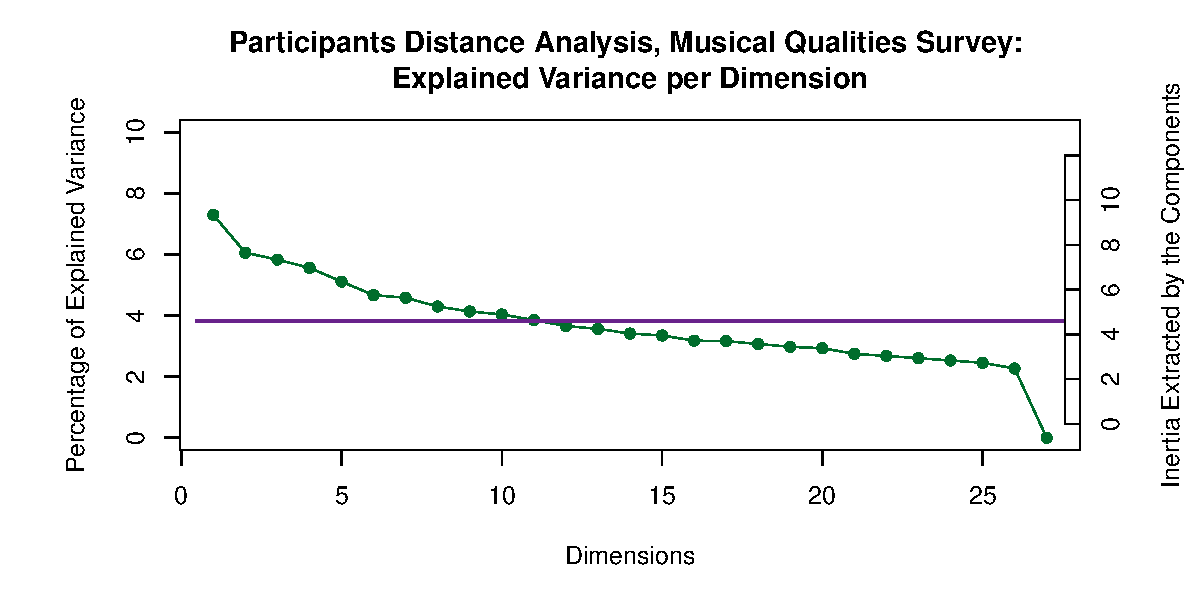
\includegraphics{Music-Descriptor-Space_files/figure-latex/screeRV-1} 

}

\caption{ }\label{fig:screeRV}
\end{figure}

\begin{figure}

{\centering 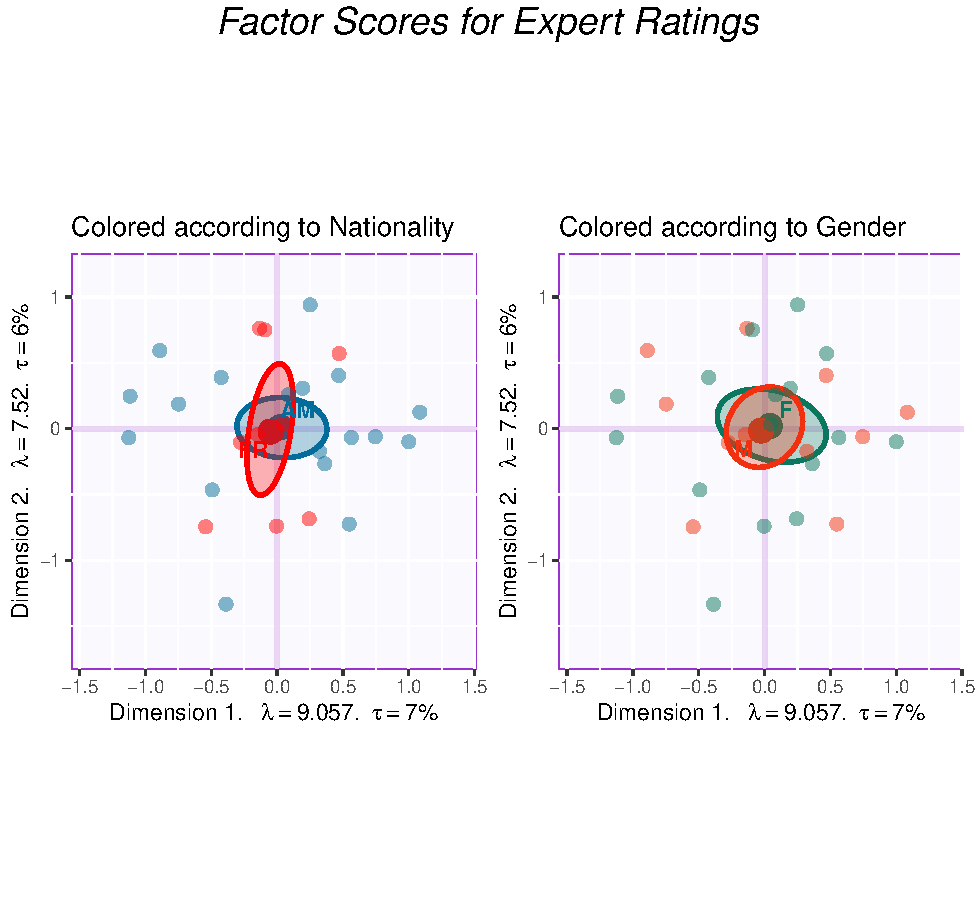
\includegraphics[width=0.5\linewidth]{Music-Descriptor-Space_files/figure-latex/judgesplot.Q-1} 

}

\caption{ }(\#fig:judgesplot.Q)
\end{figure}

\hypertarget{excerpts}{%
\subsubsection{Excerpts}\label{excerpts}}

The scree plot for the analysis of the musical quality ratings survey, \ref{fig:scree4excerptsq}, shows the high dimensionality of this space, with the first three dimensions extracting a total of 18.44\%, 14.09\% and 8.81\% respectively, totaling only 41.34\% of the variance. It isn't until we get to the 11th dimension that we see \textgreater80\% of the variance explained. However, given that the assumption in an analysis like this is that the sample is random, it's important to take these numbers with a grain of salt. Music itself is not random, and in a single excerpt of music of the type that was presented in this study, repetition is common, and some musical qualities are inextricably linked, for example some stylistic elements with genre.

\begin{figure}

{\centering 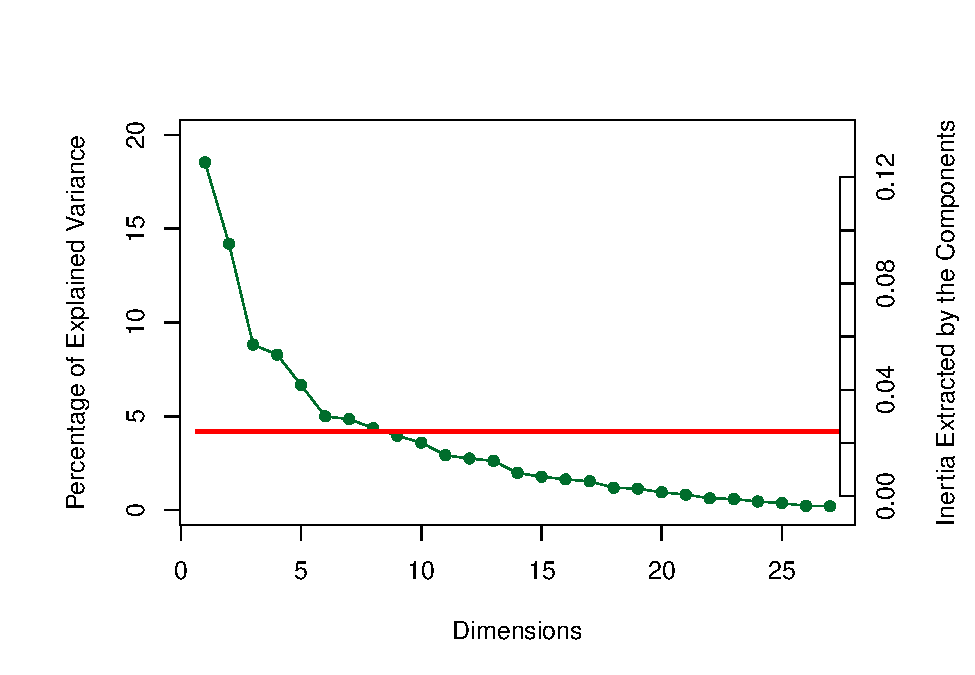
\includegraphics{Music-Descriptor-Space_files/figure-latex/scree4excerptsq-1} 

}

\caption{ }\label{fig:scree4excerptsq}
\end{figure}

Graphing the variable loadings (see \ref{fig:contributionsQ}) of the musical qualities shows which ones contribute the most to the first two dimensions. Because of how CA is calculated, we know that the excerpts that load on the same dimension and direction as the musical qualities are the excerpts that are most associated with those qualities. The contributions shown here are only those that contribute significantly to the first two dimensions.
There are some obvious groups of variables, especially tempo and articulation in the first dimension, with fewer contributions from the dynamics group. The tempo variables, which are a continuum, load from high (tempo.F6 and tempo.F7) in the positive direction to low (tempo.F2 and tempo.F1) in the negative direction. Other contributions are one-off: major harmony, triple meter, classical genre, undulating contour, and disjunct motion. The excerpts that load positively, and are therefore associated with the qualities that load in the positive direction, are all from group 2: Excerpts 4, 13, 23, and 26. The ones that load in the negative direction are from mostly from group 4: Excerpts 7, 10, 24, and 27, with one from group 3, Excerpt 3.\\
The second dimension seems to dominated by a few groups: harmony, meter, genre, dynamics. The one-offs are slow tempo, ascending contour, and ``no melody.'' The excerpts that load significantly on this dimension are from all four groups. In the positive direction, it's Excerpts 7, 12, 15, and 27 from Group 4, and Excerpt 19 from Group 1. In the negative direction it's Excerpts 2, 3, 11, and 17. All are from group 3 except for Excerpt 2, which is from Group 2. For a full enumeration of contributions, loadings, and boostrap ratios, see table {[}insert table number, also, make up table.{]} in the supplementary materials.

\begin{figure}

{\centering 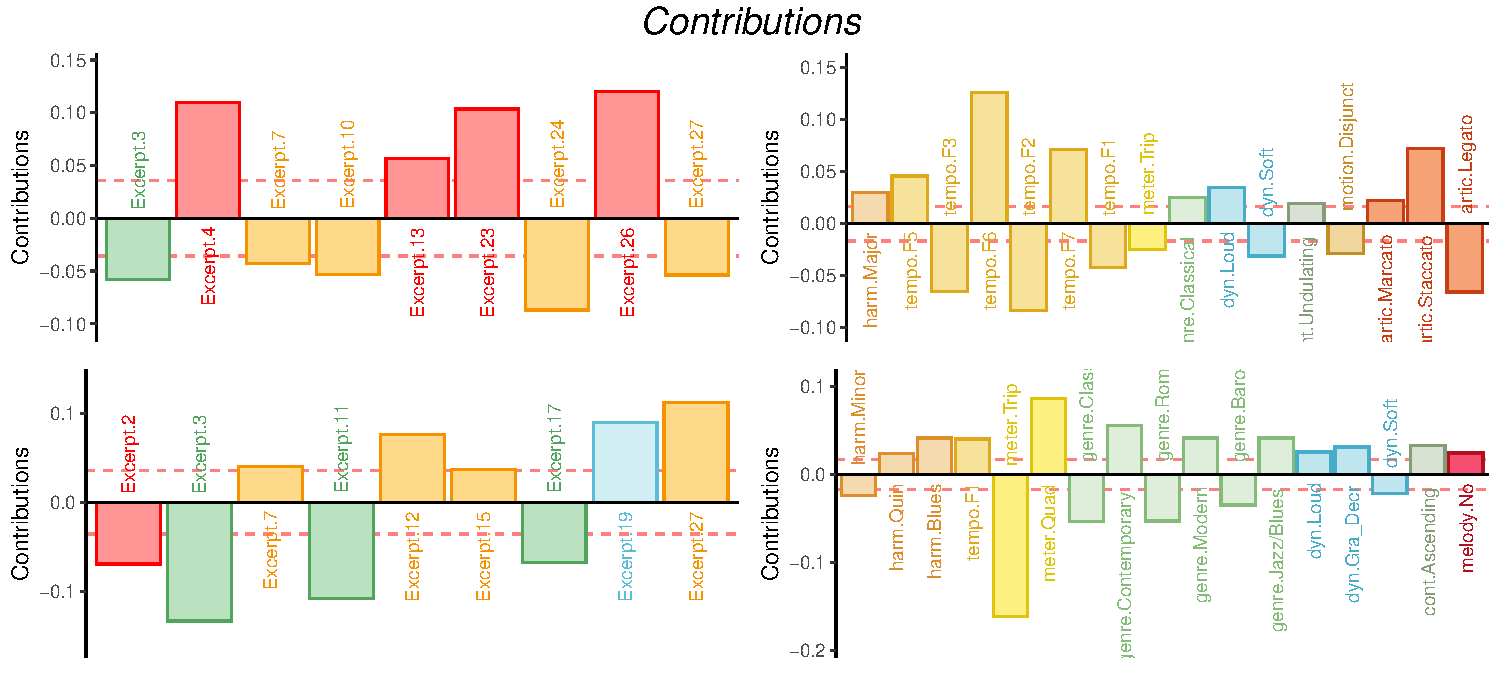
\includegraphics{Music-Descriptor-Space_files/figure-latex/contributionsQ-1} 

}

\caption{ }\label{fig:contributionsQ}
\end{figure}

\hypertarget{discussion}{%
\subsubsection{Discussion}\label{discussion}}

The graph depicted in \ref{fig:factormapswsimplexQ} is a biplot depicting how excerpts and variables plot in the same space. This biplot is possible because of the nature of correspondence analysis. Because the rows and columns of the contingency table X by definition have the same variance, the eigenvalues extracted from X are the same as X\^{}T. Thus the axes on which the factor scores are plotted are the same for both the rows and the columns. However, interpretation requires some discernment. The distance between the excerpts can be interpreted directly as similarity, and the distance between the musical qualities can be interpreted directly as similarity, but the distance between a quality and an excerpt cannot. Instead, the angle between an excerpt and a quality is indicative of their correlation. An angle of 0 indicates a correlation of 1, an angle of 90 indicates a correlation of 0, and an angle of 180 indicates a correlation of -1.\\
Overall, this helps us to evaluate what contribute to the excerpt groupings. These first two dimensions suggest that the hierarchical cluster analysis \emph{{[}see supplementary materials{]}} revealed groupings roughly according to genre. However, there are two notable outliers. Excerpts 6 and 14 are unique in that they are each the only representative of their respective genres. Excerpt 6 is minimalist, a la Steve Reich, and Excerpt 14 is jazzy. Preliminary versions of this analysis showed that they dominated the 2nd and 3rd dimensions, respectively (see supplementary materials for visualizations). In the plot below, they are included instead as supplementary projections, essentially `out of sample' elements. Their placement on the plot below alludes to the fact that the dimensionality of this space may in fact be related to musical genre or family. Although they dominated the space when included in the sample, they are much closer to the barycenter of the plot when included as out of sample. Were they to fall exactly on the origin, that would suggest that they shared no information whatsoever with the other excerpts included in the analysis. The disparity between their placement on the graph below and their placement on the graphs in which they are included in the main sample suggests that they share some information, but there is still a large amount of information that is not accounted for in the factor space below.\\
One perceptual element that is revealed here is that tempo and dynamics seem to contribute, intensity-wise, similarly to the first dimension. This points to two specific things. Firstly, it highlights possible bias in the compositional process. The excerpts were not intentionally composed with those characteristics being similar in mind, but it's entirely possible that the high or low arousal levels of the various excerpts that participants respond to also drove some of the compositional process, and that turned up in the results. Secondly, it's possible that the level of arousal was conflated between various musical qualities. For example, given two excerpts of similar tempo, one may have been rated slightly faster if it was also louder, and the other slightly slower if it was quieter. Likewise, given excerpts of similar volume, a faster one may have been rated louder than a slower one. Perception of tempo is also affected by note rate, which is also tied to arousal. In two pieces played at the same tempo, the one with more notes per unit time is more likely to be judged faster than one with fewer. {[}citations for all of this{]}
There are also a few musical elements revealed from the associations. The term staccato means short or light and separated, and the term legato means smooth and connected. The participants in this experiment didn't have access to the notation, so they would be judging the excerpts aurally only. Between faster and slower excerpts, notes of the same rhythmic value take up less time in the faster excerpts, and may be more likely to be judged as light and separate, regardless of what the actual articulation was. Slow tempo and legato are associated differently. In terms of performance practice or pedagogy, slow notes are often intended to be connected as smoothly as possible, in order to create a sense of continuity. In terms of genre and harmony, while jazz/blues (on the third dimension) is the most extreme example of this, many genres have harmonies associated with them. For example, the classical genre has fairly structured rules for both harmony and voice leading, but the romantic era relaxed those rules and introduced more complex harmonies. The gradual devolution of those rules and the increase in complexity of harmony continued through the modern and contemporary styles. Although these specific contributions aren't as strong as some of the others, a glance back at the factor scores plot shows that the older styles: baroque, classical, and romantic, are both negative on the 2nd dimension, as are the simpler harmonies of major and minor. Likewise the newer western styles: impressionist, modern, and contemporary, load positively on the 2nd dimension, along with the more complex harmonies of chromatic, whole tone, and ambiguous. Historically speaking, the whole tone scale gained great popularity with composers in the impressionist era.
However, because of the nature of this survey, this tells us more about the excerpts specifically than the behavior of the participants. Because the excerpts were composed with the intent of varying across all of these musical dimensions, what we see is a sort of validation that there is, in fact, that variety among these excerpts, and that they are different enough to create a large and varied factor space.

\begin{figure}

{\centering 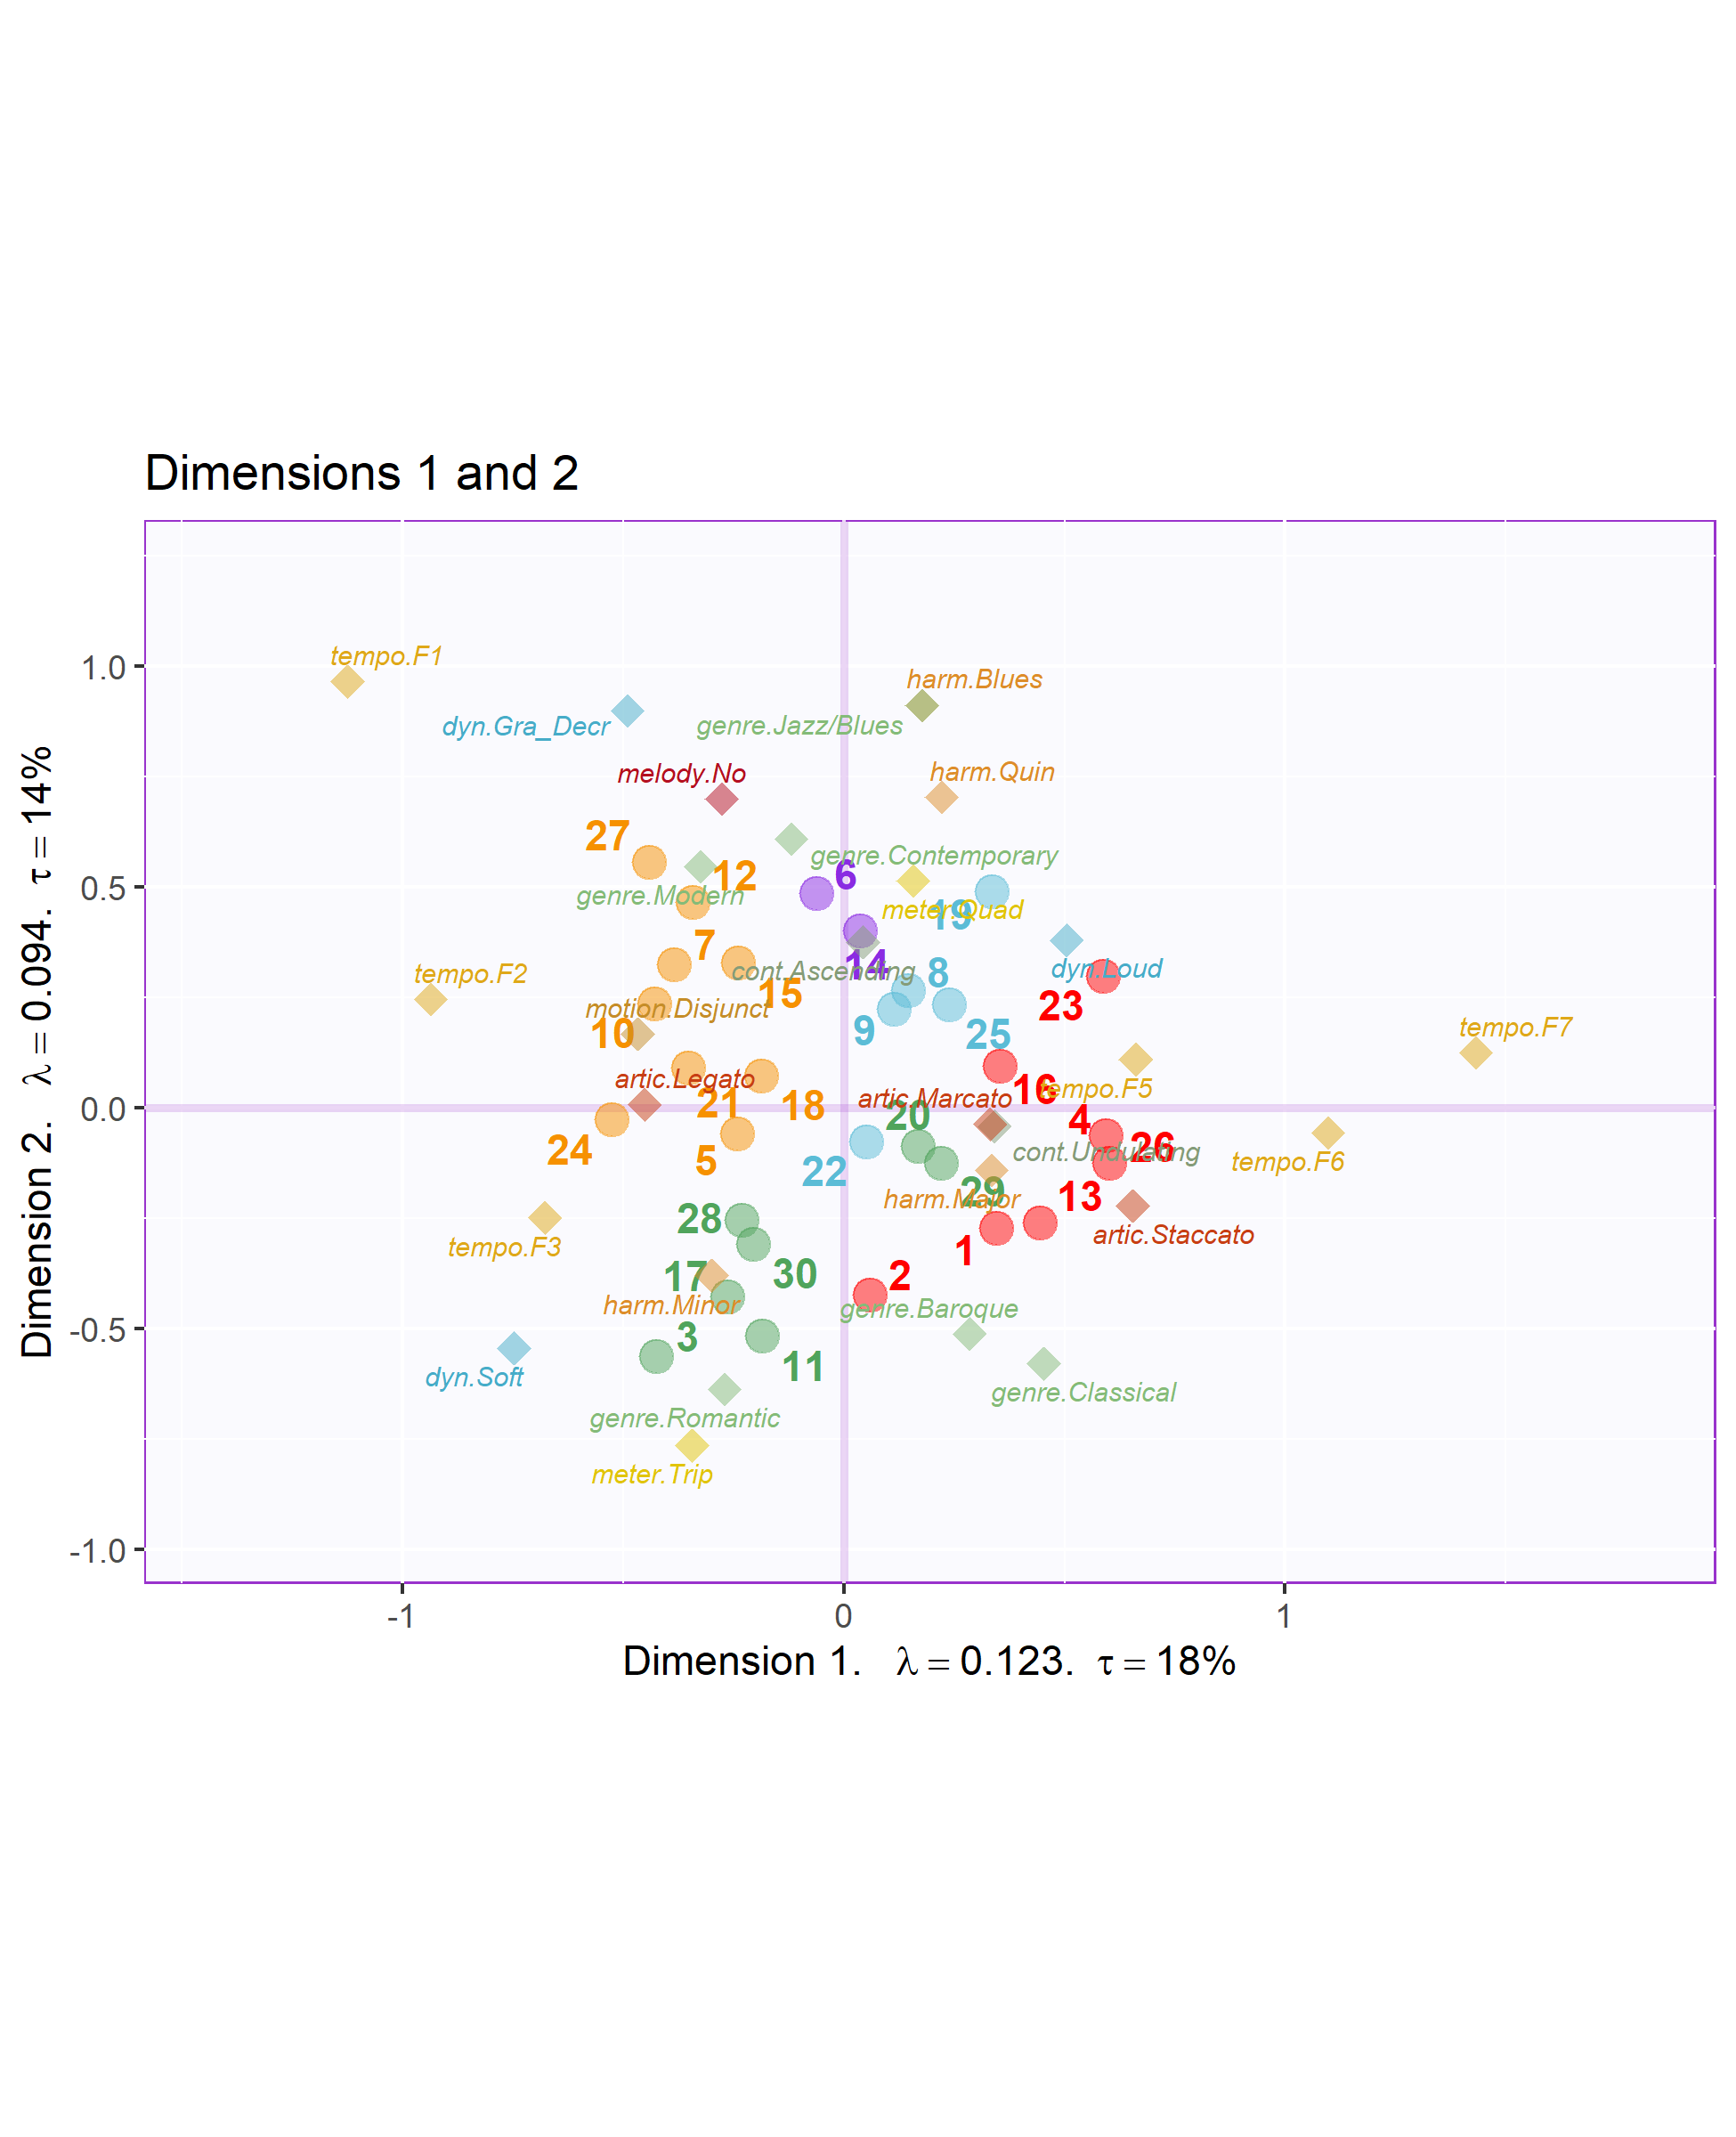
\includegraphics[width=1\linewidth]{Music-Descriptor-Space_files/figure-latex/factormaps.Q-1} 

}

\caption{ }(\#fig:factormaps.Q)
\end{figure}

\hypertarget{experiment-2-musical-adjectives-survey}{%
\subsection{Experiment 2: Musical Adjectives Survey}\label{experiment-2-musical-adjectives-survey}}

\hypertarget{participants-2}{%
\subsubsection{Participants}\label{participants-2}}

The scree plot depicted in @ref(fig:a.part.scree) shows the explained variance per dimension for the distance analysis of participants in the adjectives survey. Again, having a high number of participants means that the dimensionality is high, and each dimension is only extracting a little bit of variance. However, the first five dimensions all have \(\lambda\) \textgreater{} 1: 1.66, 1.27, 1.13, 1.09, and 1.06, respectively. However, because of the high dimensionality here, the first dimension extracts only \textasciitilde3\% of the overall variance, the second dimension extracts only \textasciitilde2\%, and each successive dimension extracts incrementally less.

\begin{figure}

{\centering 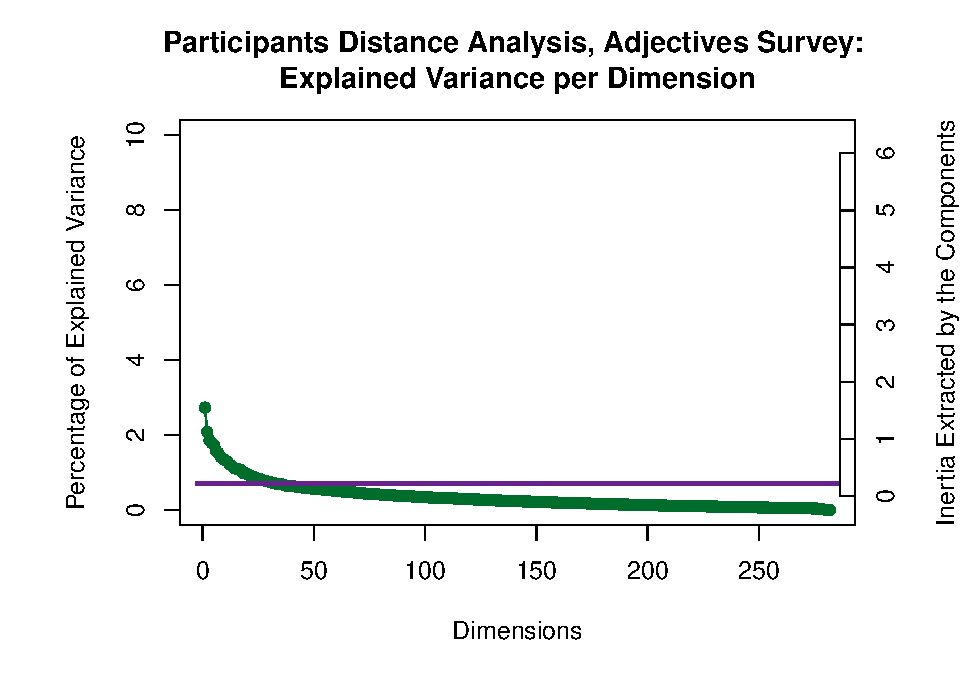
\includegraphics{Music-Descriptor-Space_files/figure-latex/a.part.scree-1} 

}

\caption{ }(\#fig:a.part.scree)
\end{figure}

MDS of a distance matrix calculated from the pages of the brick revealed significant group differences in how French and American participants described the excerpts, \(\textit p\). \textless{} .01. The factor scores of the participants are plotted below, with with group means and bootstrapped confidence intervals shown for those means. The bootstrapping resampling was performed with 1000 iterations. We also analyzed the dating using two other participant groupings as factors: gender identity, with three levels: Male, Female, or Non-Binary, and level of music training, with three levels: \textless{} 2 years, 2-5 years, and \textgreater5 years. Neither of these analyses revealed any significant differences between groups.

\begin{figure}

{\centering 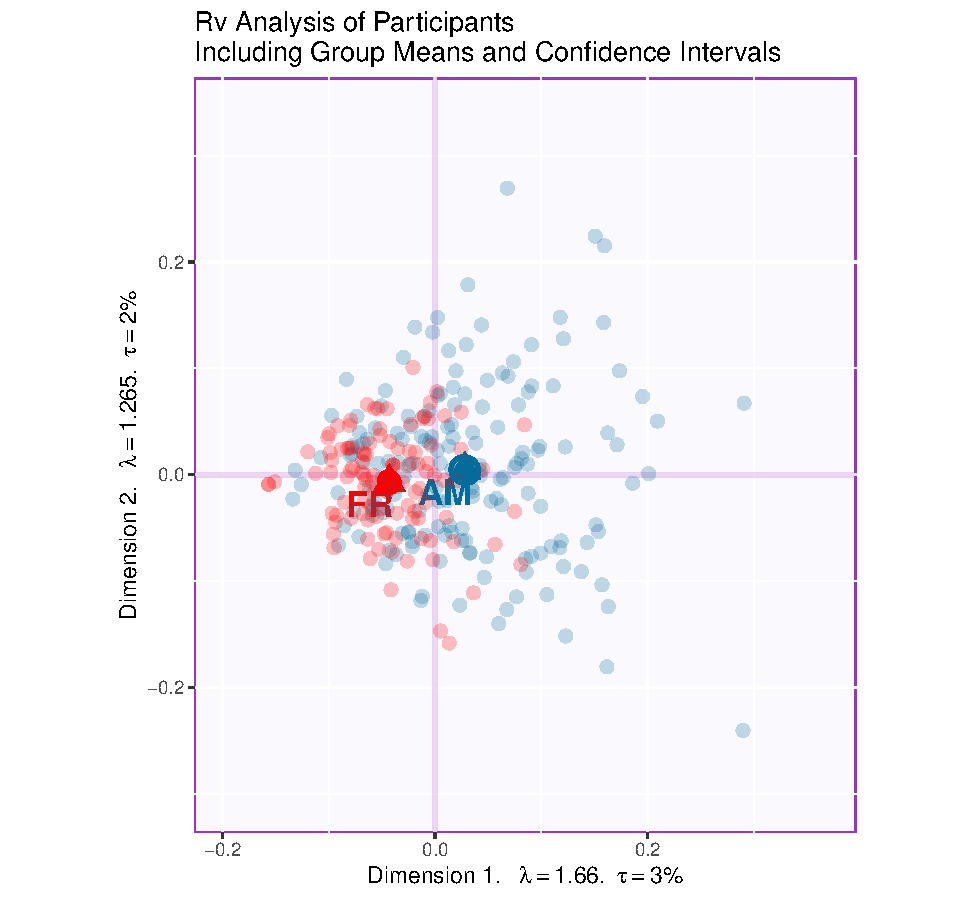
\includegraphics{Music-Descriptor-Space_files/figure-latex/map4RV.A-1} 

}

\caption{ }(\#fig:map4RV.A)
\end{figure}

\hypertarget{excerpts-1}{%
\subsubsection{Excerpts}\label{excerpts-1}}

The plot below shows the explained variance per dimension in the analysis of the excerpts contingency table. Although there are no components with \(\lambda\) \textgreater{} 1, there are two strong dimensions that extract a majority of the variance. The first two dimensions extract 72.25\% of the variance, with the first dimension extracting a majority: 50.05\%, and the second dimension extracting almost a quarter of the overall variance: 50.05\%. This plot also suggests that there are multiple `elbows,' at the 3rd, 5th, and 7th dimensions, respectively, with the third and fourth dimensions forming an `eigen-plane,' of two dimensions which extract similar amounts of variance and should be considered together. For this analysis, however, we're focused on the two first dimensions.
Although excerpts 6 and 14 are outliers in the musical qualities survey, for reasons detailed above, they were not outliers in this analysis. We therefore included them in all of the analyses for Experiment 2.

\begin{figure}

{\centering 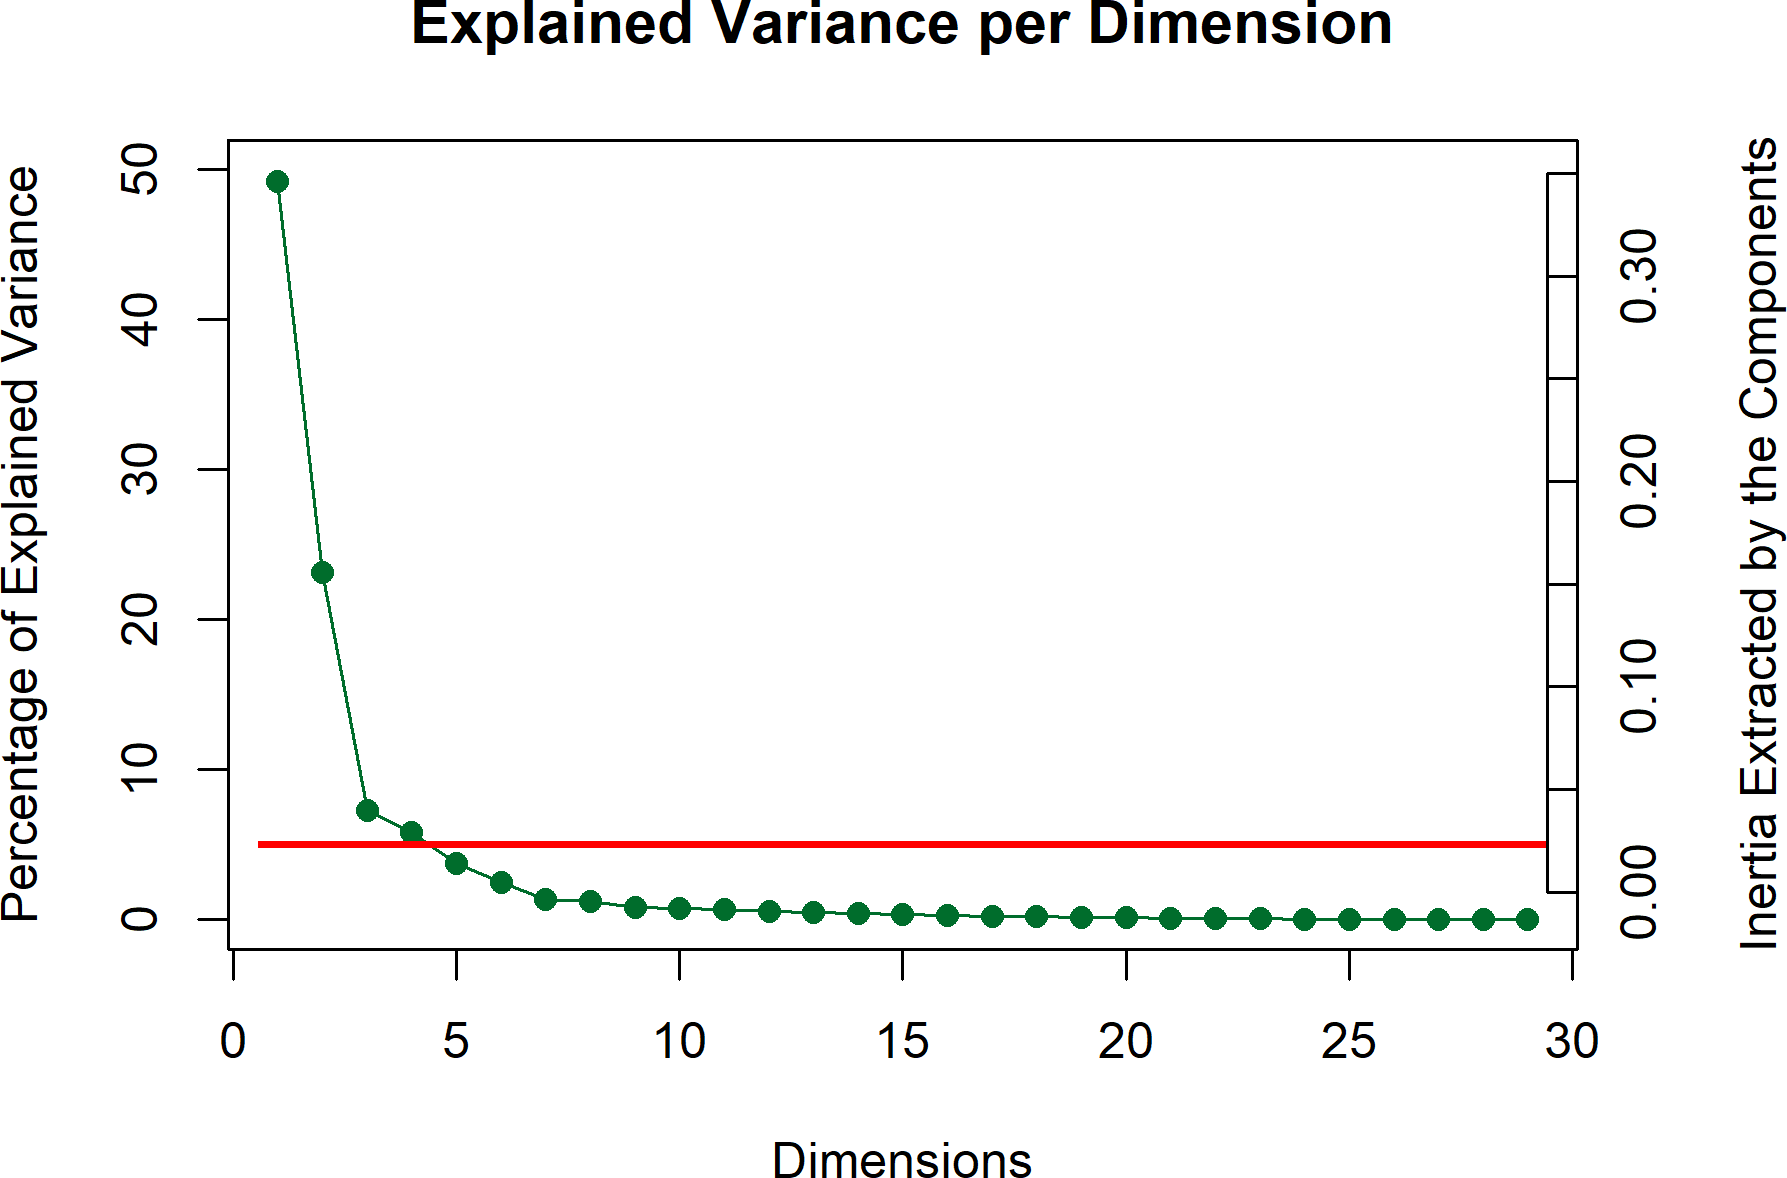
\includegraphics{Music-Descriptor-Space_files/figure-latex/scree4descriptors-1} 

}

\caption{ }\label{fig:scree4descriptors}
\end{figure}

Contributing significantly to the positive end of the first dimension are excerpts from group three (green) and to the negative end are excerpts from group one (yellow). Strong contributions on the positive end of the dimension from the adjectives ``Sad,'' ``Dark,'' ``Melancholy,'' ``Slow,'' ``Mysterious,'' ``Solemn,'' and ``Disturbing.'' The negative end of the first dimension is defined by the adjectives ``Fast,'' ``Happy,'' ``Dancing,'' ``Colorful,'' and ``Bright.''
The second dimension is dominated by excerpts from group 4 (red) in the positive direction and group 2 (blue) in the negative direction. Two excerpts from group 3 also contribute significantly, excerpts 7 in the positive direction and excerpt 10 in the negative direction. The columns contributing strongly in the positive direction are ``Aggressive,'' ``Fast,'' ``Disturbing,'' ``Mysterious,'' ``Surprising'' and ``Complex.'' The columns contributing in the negative direction are ``Warm,''Soft``,''Happy``,''Slow``,''Round``, and''Light".

\begin{figure}

{\centering 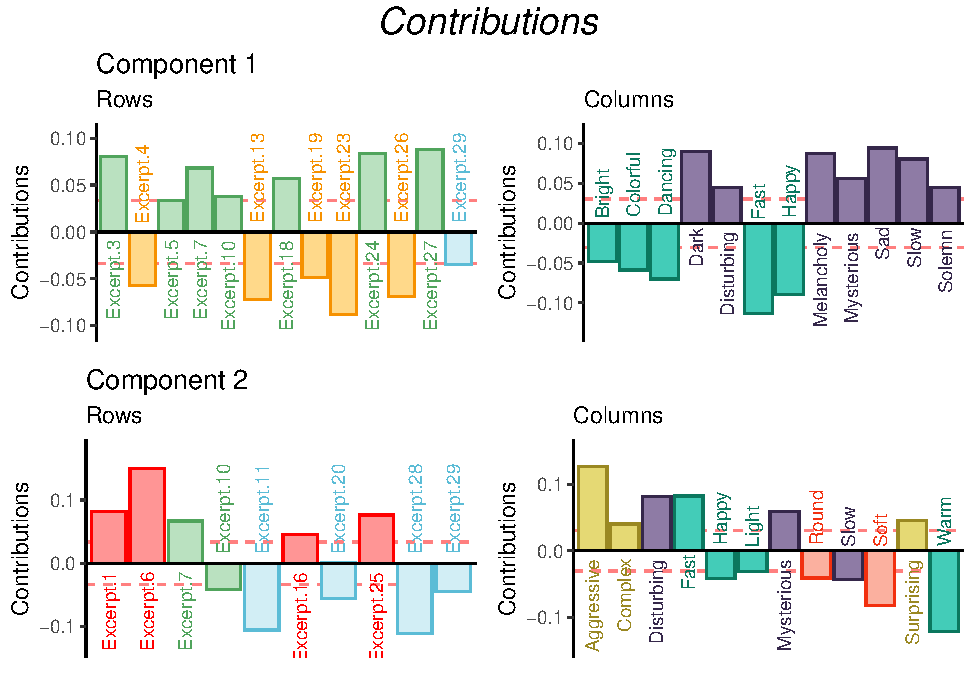
\includegraphics{Music-Descriptor-Space_files/figure-latex/contributions.A-1} 

}

\caption{ }(\#fig:contributions.A)
\end{figure}

The barplots in @ref(fig:theboots.A) show the bootstrap ratios calculated for the rows and columns. Here we've included all of the rows and columns, because it's useful to see both which are significant and which are not. This is an inferential method that tells us is how consistently each of the observations and variables load on the first two dimensions. The threshold in this case is \emph{p} \textless{} .05. From this we get an idea of which of the rows and columns are stable, in other words, which ones tended to be rated in a certain way consistently across all participants, and also how likely these are to be observations reflective of the population as a whole. In this plot, the more extreme value of the bootstrap ratio, the more likely that it is a reflection of the `real' value. The values in the center of each plot that are grayed out identify the rows or columns that are not consistently loading on the dimensions. With the observations and variables ordered like this, it makes it easy to see how the consistently the clusters are distributed in the space. This plot was not included for experiment 1 because it would be less informative given what the survey in experiment 1 was assessing. Experiment 1 doesn't evaluate the behavior of participants, but the nature of the excerpts.
Note that there are far more significant bootstrap ratios than there are significant contributions. That just means that while not everything is contributing, overall the model seems to be stable. Fewer significant bootstrap ratios would suggest that there was a greater amount of variance in the observations and variables than were accounted for, at least in the first two dimensions. Looking at the nonsignificant values for the adjectives may inform our understanding of the participants' use of the adjectives. `Incisive,' `transparent,' `poweful,' `dense,' `round,' and `sparse,' are all nonsignificant on the first dimension, and `weak,' `dull,' `sparse,' `valiant,' and `short' are all nonsignificant on the second dimension. All but `sparse' are significant on one dimension or the other. Looking at the column sum for `sparse' tells us that it was used, so this isn't an effect of participants not using this word. It's more likely that `sparse' doesn't really fit into the Valence-arousal plane. It's a neutrally valenced word that could describe excerpts that fall anywhere within that plane. `Weak' and `transparent' give us another important perspective. These were the two least commonly used adjectives, but the fact that they are consistently loading on one dimension or the other suggests that when they were used, they were used in the same way.

\begin{figure}

{\centering 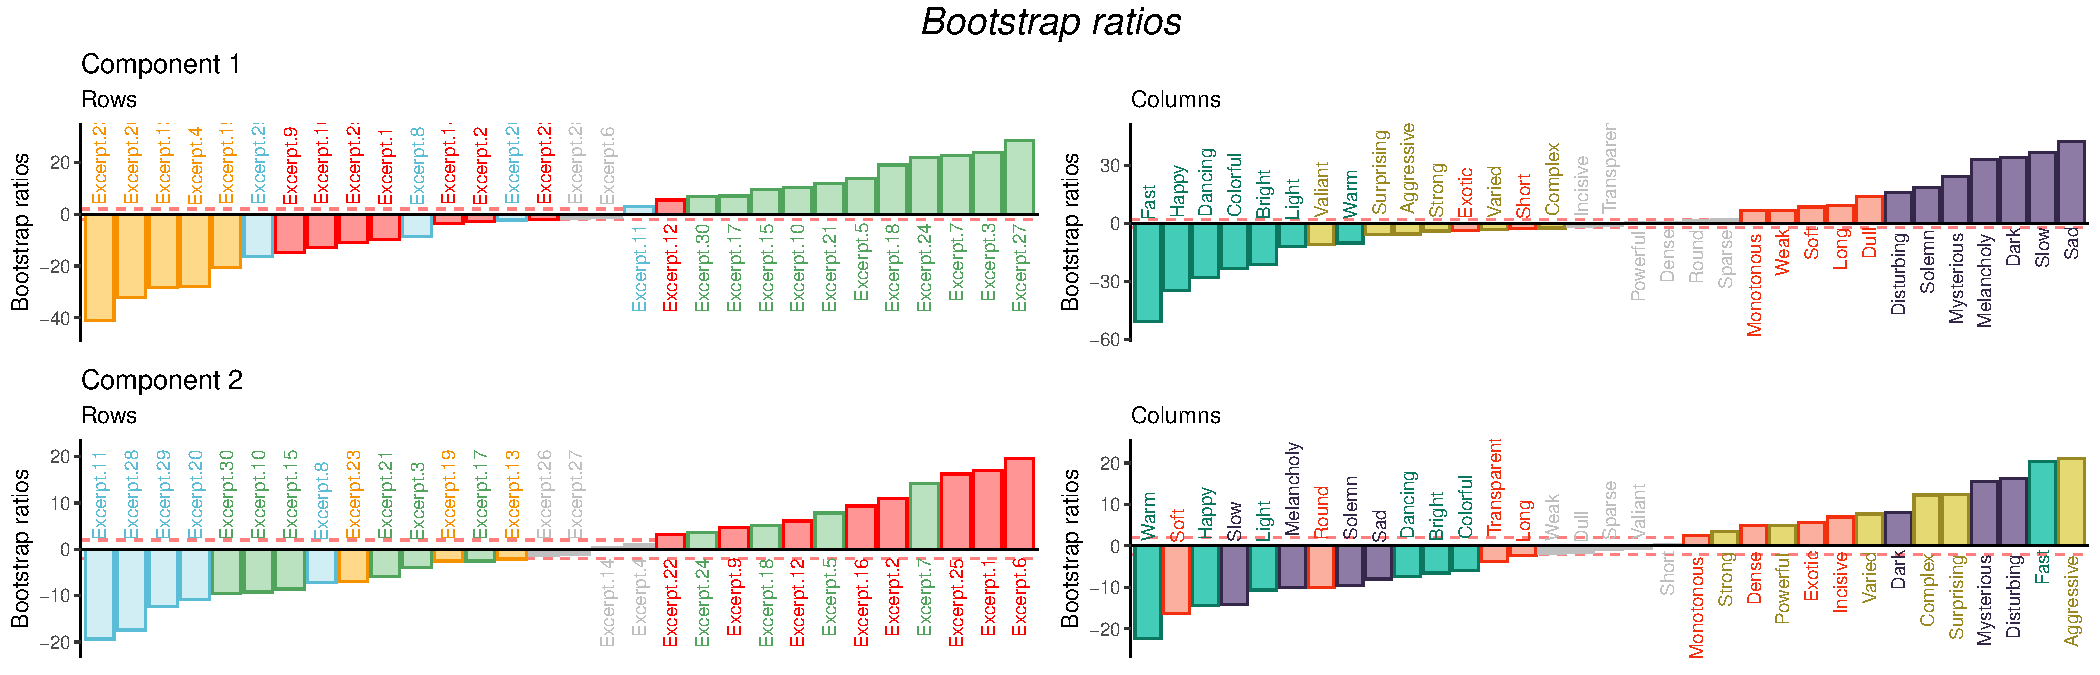
\includegraphics{Music-Descriptor-Space_files/figure-latex/theboots.A-1} 

}

\caption{ }(\#fig:theboots.A)
\end{figure}

\hypertarget{discussion-1}{%
\subsubsection{Discussion}\label{discussion-1}}

The factor maps below show the row and column factor scores for the american and french participants. These are once again symmetric plots, interpretation is the same as the factor plot for the musical qualities. There's a clear valence-arousal plane apparent for both, and in both cases valence seems to define the first dimension and arousal defines the second dimension. However, the difference in the amount of variance extracted by the first two dimensions between the french and american participants is notable. The french data show a weaker first dimension but a stronger second dimension relative to the americans, both in terms of variance extracted (tau), effect size (lambda). This tells us that french participants were less affected by the excerpts than the american participants, but they responded more to the arousal of the excerpts.
There are also differences in how the adjectives and the excerpts are distributed in the space. One clear example is that Excerpt 6 is in quadrant two in the american plot, but quadrant one in the french. This is a small change, but it suggests that the french participants were more likely to assign negative valence to this excerpt, and American Participants were more likely to assign positive valence. For the adjectives, `bright' and `dancing' are directly on top of one another in the American plot, but there is some space between the two in the French plot. It's possible that this reflects the idea that although the meaning is shared between languages, there are semantic or associational differences between the words.

\begin{verbatim}
## [1] "Preprocessed the Rows of the data matrix using:  None"
## [1] "Preprocessed the Columns of the data matrix using:  Center_1Norm"
## [1] "Preprocessed the Tables of the data matrix using:  MFA_Normalization"
## [1] "Preprocessing Completed"
## [1] "Optimizing using:  None"
## [1] "Processing Complete"
\end{verbatim}

\begin{verbatim}
## [1] "Preprocessed the Rows of the data matrix using:  None"
## [1] "Preprocessed the Columns of the data matrix using:  Center_1Norm"
## [1] "Preprocessed the Tables of the data matrix using:  MFA_Normalization"
## [1] "Preprocessing Completed"
## [1] "Optimizing using:  None"
## [1] "Processing Complete"
\end{verbatim}

Additionally, a post-hoc Multiple Factor Analysis revealed the following in terms of the semantic and perceptual differences between French and American participants.

\begin{figure}

{\centering 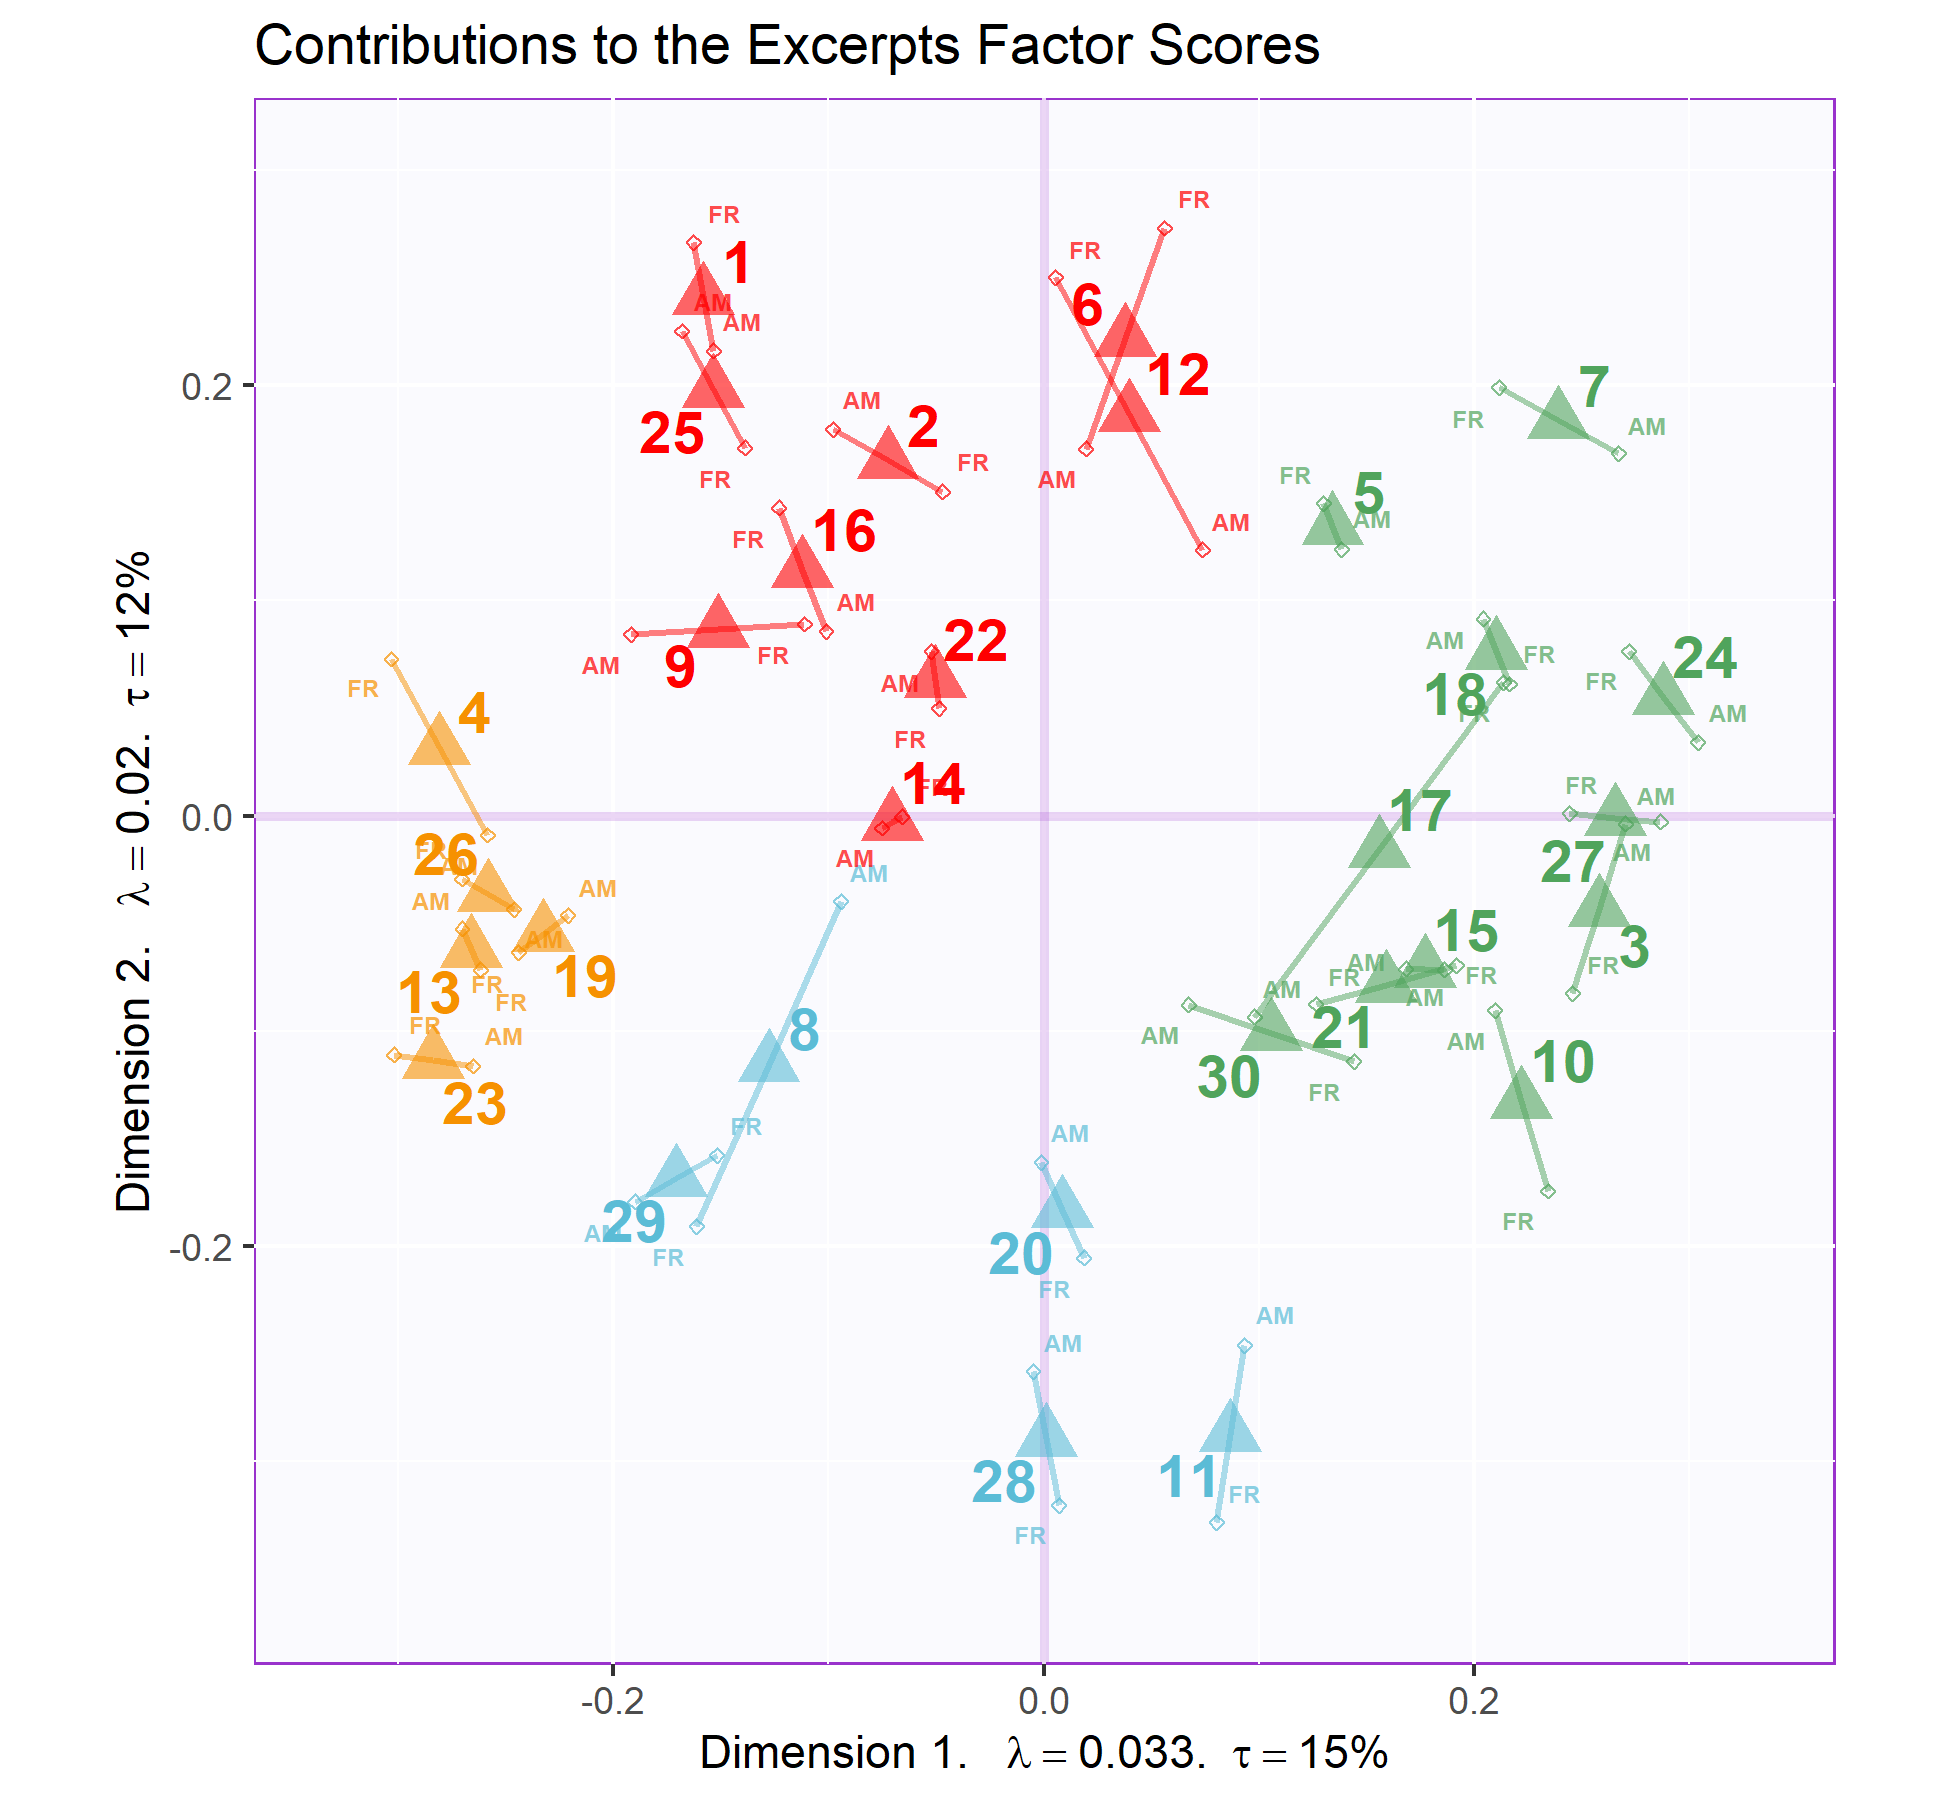
\includegraphics{Music-Descriptor-Space_files/figure-latex/mfasbs-1} 

}

\caption{ }\label{fig:mfasbs}
\end{figure}

\hypertarget{experiment-3-combined-surveys}{%
\subsection{Experiment 3: Combined Surveys}\label{experiment-3-combined-surveys}}

Experiment 3 used the pseudo-contingency tables from experiments 1 and 2 together. Since excerpts 6 and 14 were excluded from analysis for experiment 1, we also removed those rows from the contingency table for experiment 2. This is so that the dimensions of the two tables for this PLSC would be conformable (remember that we need the same rows or columns in both tables for this analysis). The point of this experiment is to identify the strongest covariance between the two tables - that is, the strongest shared signal between two data tables. Now, this is not to say that these two tables are evaluating the same thing. Instead it allows us to see what is most common between two sets of different information - how often an excerpt was associated with \emph{both} a musical quality and an adjective. The visualizations below allow us to see which variables from each of the two tables correspond with one another; which adjectives are associated with which musical dimensions. Even though both individual tables have their own factor spaces, plotting the common factor space between the two should allow us to see which excerpts are separated from one another using data from both surveys.

\hypertarget{results-1}{%
\subsubsection{Results}\label{results-1}}

This analysis revealed two dimensions that extracted the majority of the variance (83.60\%). Of that total extracted by the first two dimensions, the first dimension extracted 64.35\% and the second dimension extracted 19.26\%. The scree plot below shows that it's possible that there are two elbows in this graph, at the 3rd and 5th dimensions. The 3rd and 4th dimensions are also significant, extracting 6.02\% and 3.67\% of the variance, respectively. Interpretations of the third dimension and beyond is beyond the scope of this paper, but seeing that there are multiple significant dimensions beyond the second does provide a possible future direction using this method.

\begin{figure}

{\centering 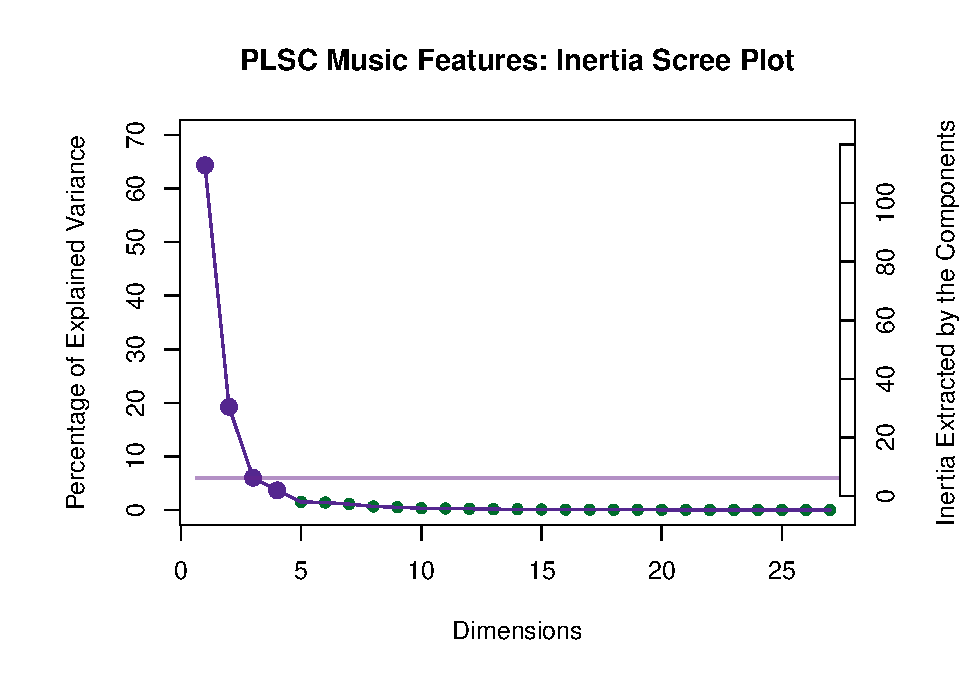
\includegraphics{Music-Descriptor-Space_files/figure-latex/screePLSC-1} 

}

\caption{ }\label{fig:screePLSC}
\end{figure}

The plot below shows which variables from each data table load the most on the first and second dimensions. For the purposes of this visualization, we are showing only the variables for which 70\% or more of the variance is explained. The nature of the PLSC also suggests that these are the variables that are most associated with one another between the two tables. The strongest signal on the first dimension juxtaposes the slow and legato musical qualities in the positive direction with the fast, staccato, marcato, and conjunct musical qualities in the negative direction. The adjectives associated with the qualities in the positive direction are ``Dark,'' ``Dull,'' ``Long,'' ``Melancholy,'' ``Sad,'' ``Slow,'' ``Solemn,'' and ``Weak.'' The adjectives associated with the negative direction are ``Bright,'' ``Colorful,'' ``Dancing,'' ``Fast,'' ``Happy,'' and ``Light.''\\
The second dimension identified in the positive direction major harmony and mezzo dynamics, associated with ``Light,'' ``Round,'' ``Soft,'' and ``Warm.'' The negative direction is driven by the impressionist genre being associated with ``Aggressive,'' ``Complex,'' ``Dense,'' ``Disturbing,'' ``Powerful,'' and ``Surprising.''

\begin{figure}

{\centering 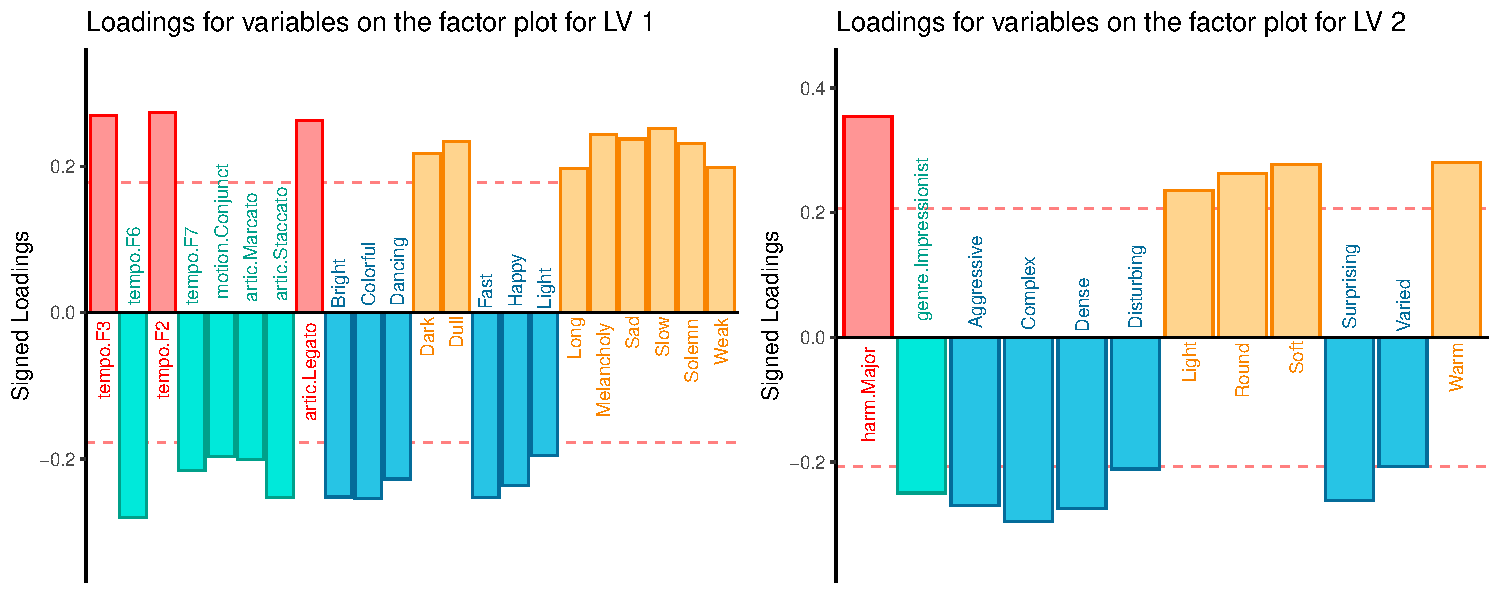
\includegraphics{Music-Descriptor-Space_files/figure-latex/loadingsplsc-1} 

}

\caption{ }\label{fig:loadingsplsc}
\end{figure}

Contributions and loadings are similar, but not exactly the same. Here were see that there are quite a few more variables that contribute significantly to these dimensions than for which a significant portion of the variance is explained. We do see similar groups, however: on the first dimension, the tempo variables are contributing significantly, along with some from harmony, density, genre, dynamics, motion, range, and articulation. The adjectives contributing significantly are Bright, colorful, Dancing, Fast, Happy, Light, and Valiant in the negative direction, and Dark, Dull, Long, Melancholy, Monotonous, Sad, Slow, Solemn, and Weak in the positive direction. What's notable here is that while some of these variables did contribute significantly in the plots above (see @ref(fig:factormaps.A) and @ref(fig:factormaps.Q)), some didn't contribute much at all and fell near the barycenter of the factor plot. We also see that this juxtaposes some negatively and positively valenced adjectives, which allows us to identify which of the musical qualities contributes to the valence dimension.
The second dimension tells us a similar story. Here we see more of the harmony variables, along with one tempo variable, some density, genre, a few dynamics, contour, motion, range, and articulation. The adjectives contributing negatively are Aggressive, Complex, Dense, Disturbing, Incisive, Mysterious, Powerful, Surprising, and Varied, and those contributing positively are Light, Round, Soft, Transparent, and Warm. Again we see similar effects of variables that may not have contributed significantly to their respective plots above, but are contributing significantly here. Also, this second latent variable seems to be defining the arousal dimension.\\

\begin{figure}

{\centering 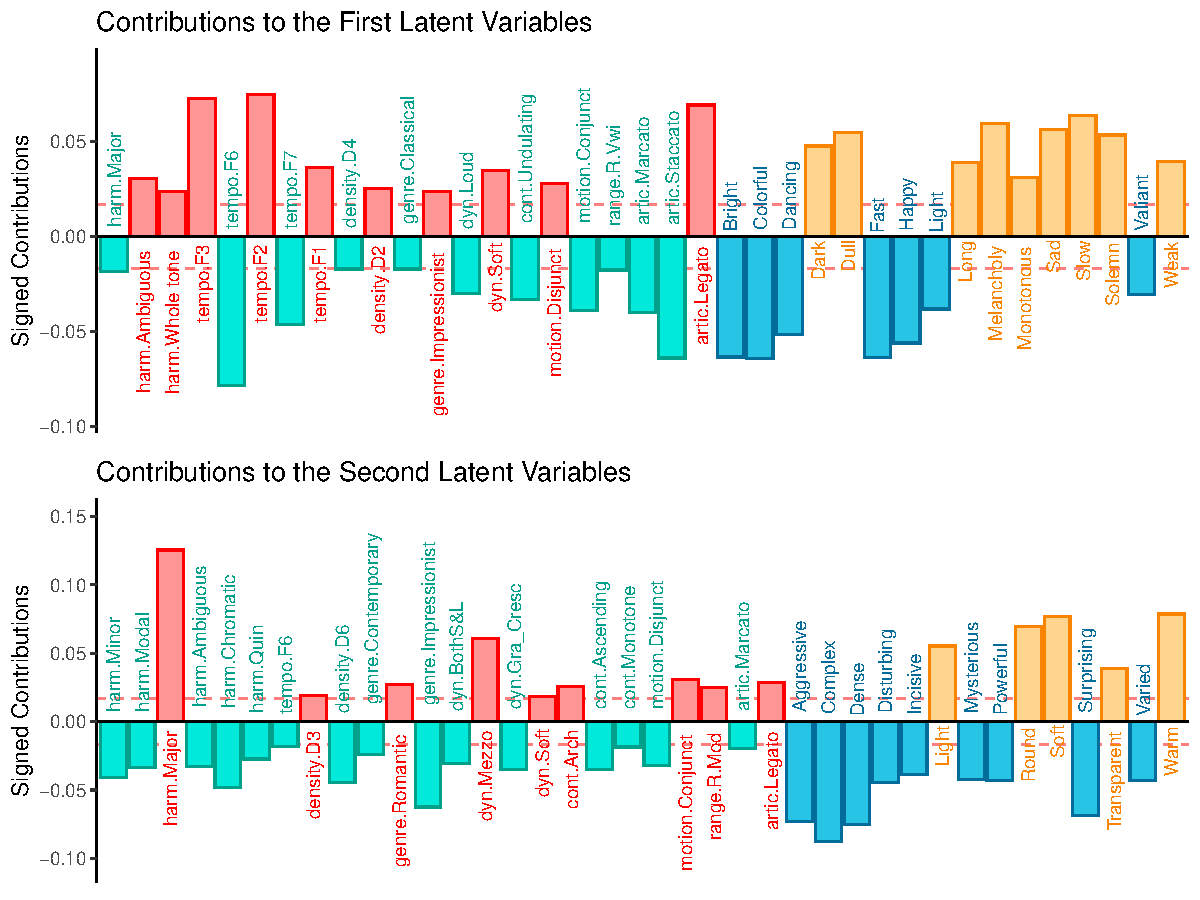
\includegraphics{Music-Descriptor-Space_files/figure-latex/contsplsc-1} 

}

\caption{ }\label{fig:contsplsc}
\end{figure}

\hypertarget{discussion-2}{%
\subsubsection{Discussion}\label{discussion-2}}

The factor score plots for this analysis shows that the first two sets of latent variables extracted by the analysis effectively separate the groups of excerpts into the clusters defined in the HCA for the adjectives survey. This factor plot shows us how the strongest correlated signal between the two data tables separates Excerpts groups 2 and 3, but groups 1 and 2 didn't contribute much to this dimension, instead contributing to the 2nd latent variables. The second latent variable separates Groups 1 and 4, with Groups 2 and 3 more barycentric. This suggests that, generally speaking, the excerpts that were clustered in groups 2 and 3 are those that could be defined by positive and negative valence, respectively, and those in groups 1 and 4 would be defined more by high and low arousal. That being said, these excerpts are not defined \emph{exclusively} along these dimensions, but rather more by one than the other. For example, excerpt 26 is characterized by being one of the most extreme examples of positive valence, but doesn't score as highly on the arousal dimension, similarly with excerpt 27 with negative valence. This is contrasted with excerpt 7, which is one of the most negatively valenced stimuli, but also scores very high on arousal, although the barycenter for that group is near the origin of that plot.

\begin{figure}

{\centering 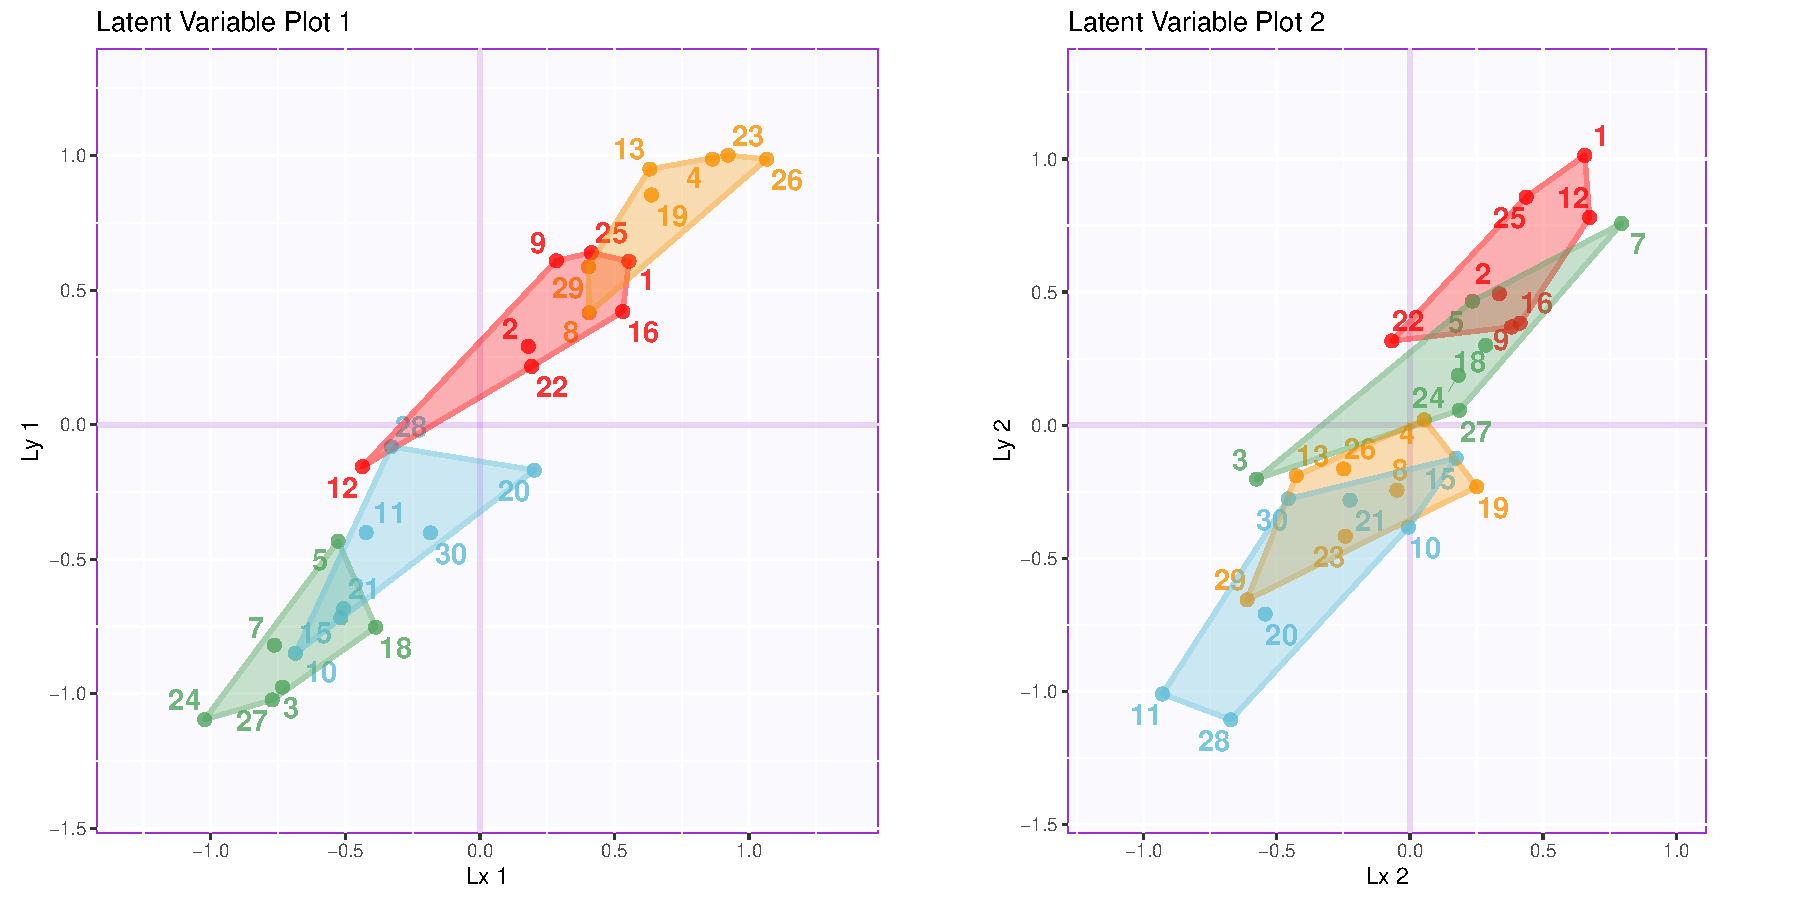
\includegraphics{Music-Descriptor-Space_files/figure-latex/factorplotsPLSC-1} 

}

\caption{ }\label{fig:factorplotsPLSC}
\end{figure}

\hypertarget{general-discussion}{%
\section{General Discussion}\label{general-discussion}}

Although this study was designed to evaluate the sensory or cognitive response to music, and not specifically the emotional response, there is significant overlap in the results observed here and the results of the work investigating music and emotion. The appearance of the valence-arousal plane in the results of experiment 2 was not unexpected, even though the adjectives we selected were not intended to be explicitly emotional. This goes to show difficult it is to avoid any emotional content when selecting descriptors, and from another perspective, how much emotional contagion the musical examples carry. Overall, this supports the idea that the first two dimensions on which music is judged holistically are valence and arousal.
Some of the results discussed in Experiment 1 require more explanation. In experiment 1, there was an issue of having two individual excerpts dominate the factor space, numbers 6 and 14, which did not happen in experiment 2. One of the ways in which CA is different from PCA is that PCA is usually unweighted. CA, on the other hand, makes use of weights and masses to find the average observation. Information that is common, therefore, falls towards the center of the plot, while information that is further from the average, in other words, more rare, ends up further from the center of the factor plots. {[}cite{]} Therefore, if a survey like the one used in experiment 1 includes a item that is wildly different than the others in the set, the ratings will be very different, and that item will dominate the factor space. In this case we have two such examples: excerpts 6 and 14. Excerpt 6 was written as a Steve-Reich-esque minimalist, ostinato based excerpt, and excerpt 14 was written to be jazzy. The reason this effect occurs with the first survey and not the second is that the musical qualities on which the excerpts were rated were explicit and designed to separate the excerpts along the various musical dimensions, while the adjectives survey was designed to evaluate the excerpts more generally on holistic qualities. Excerpt 6 still appears as a minor outlier in the visualizations for the second survey, but does not dominate the space the way it does in the results of the first.
What we did to mitigate that is to use those two excerpts as \emph{supplementary projections}, sometimes also referred to as \emph{out of sample observations}. This allows us to evaluate what information is shared by those outliers with the other elements in the dataset without having them dominate the visualization of the factor space. If, when we projected those values into the factor space, they projected onto the origin or very close to it, we would know that those observations shared no information with the other variables. The fact that they are where they are offers support to the idea that the first survey separates the excerpts approximately by genre. Because the `genre' information isn't shared with the other observations, they are being projected onto the space sharing only the information that does not deal with genre, like tempo or range. What this tells us is that musical qualities surveys captured a result that may have characterized by 4-6 factors, each approximating genre and the qualities associated with that genre and the general affective space captured an entirely different set of information about the stimuli and the perception of the stimuli.\\
The hierarchical cluster analyses revealed different groupings in how the stimuli were rated between the two surveys. The PLSC then showed that when including both sets of data, there was a coherent interpretable factor space on which the excerpts were plotted. There are a number of ways to further disambiguate the results of the surveys. One way would be to run a MFA, similar to the one above that plotted the difference between French and American raters on the adjective survey. This would allow for a number of different interpretations. Firstly, it would calculate the overall factor space for the excerpts, including all of the data from both surveys, without separating out the first and second dimensions to plot them separately. It would also identify the specific partial factor scores for each of the data tables within that factor space that would allow for the interpretation of the relative differences between the data tables. The drawback to both of these, however, is that unlike the separate correspondence analyses we ran above, where the row and column scores can be plotted in the same space, neither MFA nor the PLSC allow for that type of visualization. That being said, because different types of analysis reveal different aspects of the data, running both analyses can provide a broader understanding of the data, and each could provide explanations for what remains ambiguous in the other.
An important overall takeaway from this is that with a deep general understanding of the stimuli, we may be able to predict the approximate dimensionality of the solution factor space. In the first survey, the solution was that the stimuli were largely separated along genre or stylistic lines. One issue that arose with this is that there was only one example of minimalist and jazz music. To have a solution in which we didn't see these specific excerpts as outliers, but as coherent members of a factor space, we would need more examples of those styles. This suggests that when creating surveys or designing stimuli, we should keep in mind that we need multiple items per group, or presumed dimension. This is not to say that we will always be able to a priori predict the factor space of the solution. For example, experiment 2 may also have benefitted from more minimalist or jazz examples - in a system in which the overall structure is obtained by evaluating the stimuli holistically, having a single outlier will necessarily distort the space. Either because it is an outlier in sensory terms or because it is the only stimulus against which there is no direct reference. This in a way embodies the issue described in the introduction, where we have a single dimension that is noisy. This really only applies to experiment 2. The noise comes from the fact that participants were likely to be less familiar with mimalism and/or jazz than the trained musicians who took the QS, but the reason the results are overall robust to that noise is that the participants were not asked to rate the excerpts on any explicit dimensions or qualities.

\hypertarget{limitations-future-directions}{%
\subsection{Limitations \& future directions}\label{limitations-future-directions}}

Although we evaluate the scores and ratings of participants from different countries, we recognize that the issue of multiculturality is not addressed to a significant degree in this study. The sample was still largely students, and France and the United States share similar musical cultures. To truly address this question, it would be very interesting to include participants from multiple, contrasting musical cultures, with languages that are more distinct than English and French. This presents new problems, however, as the specific musical qualities included in the surveys may not all apply to or translate well to other musical cultures. Harmony, for example, is a concept that is developed to a significant degree in western music, but melody or rhythm may be the fundamental focus of other musical cultures (cite patel here? I forget.).
Another question that fell beyond the scope of this study is the concept of semantic drift between languages. Although illustrated in \ref{fig:mfasbs}, the source of the differences between French and American participants is not entirely clear. We humbly hazard to guess that some of the sources of the difference include aspects of perception that extend beyond the musical. These could be linguistic sources, such as the physical characteristics of the words themselves, the cultural associations with the words, or the frequency of use in either language. Diving more into those questions of linguistics and semantic drift between languages would be a fascinating future study.
Another interesting study would be to repeat this study using adjectives from specific domains or that that avoid explicit emotional or musical content, to see how music maps onto different sensory spaces. For example, `moist,' `slimy,' `dry,' `puckered,' `smooth.' Although some of these adjectives may carry musical weight, in the context of other words that all relate to haptic sensation, it may provide some interesting feedback regarding how the music maps into other sensory domains.
Finally, using these studies may provide pilot work for the way in which people without language react to music, nonverbal autistic people, for example. Whereas this study explicitly uses language as an interlocutor for music perception, it offers insight into ways to better communicate with people who do not have that ability.

\hypertarget{conclusions}{%
\section{Conclusions}\label{conclusions}}

By developing investigative paradigms that are accessible on mobile platforms and that reduce participant demand while maintaining rigor and integrity, we are likely to be able to reach a much greater subset of the population. If we are able to pair this kind of data gathering with appropriate analysis, we can maintain the standards of scientific integrity that we as a community expect with traditional hypothesis testing. The literature to date in the music cognition domain has focused on a fairly small subset of the multivariate analyses available to investigate these questions. As presented here, the number of ways that exist to analyze the data from a single set of experiments is considerable, and the results of each analysis illuminate different parts of the story the data are telling. Not every form of analysis is appropriate in every context, but understanding how, and perhaps more importantly when, to apply a technique or type of analysis is an important to uncovering new perspectives or insights.

\newpage

\hypertarget{references}{%
\section{References}\label{references}}

\begingroup
\setlength{\parindent}{-0.5in}
\setlength{\leftskip}{0.5in}

\hypertarget{refs}{}
\begin{CSLReferences}{0}{0}
\end{CSLReferences}

\endgroup


\end{document}
